\section*{Contents of the dissertation}

% Is there no way to pull the chapter numbers from the main document? 
\textbf{Introduction} presents the background and basic context, outlines the whole thesis. Specifically, it underscores the relevance of the conducted research: the proposed algorithms and approaches are widely applicable, including power systems operation due to the emerging renewable energy integration into the power grids. Next, it describes the current state of the field, explains the problem in current developed approaches and reveals the research gap. Further, it states the aims of the dissertation, shortly, this work aims at increasing efficiency of the data-driven algorithms in stochastic optimization setting applied to power systems context. The scientific novelty is covered by applying advanced statistical methods and novel approaches that increase an efficiency of existing data-driven approaches in stochastic optimization. Additionally, the introduction underscores practical and theoretical significance: current dissertation addressed the theoretical gap in methodologies for reduction of data usage, the practical significance is demonstrated by applicability of proposed methods for real world application - power systems operation. Finally, the introduction covers methodology, propositions for defence and approbation together with reliability.

%introduces the necessary definitions and ideas of quantum computation. Section 1.1 introduces quantum states, unitary, Hermitian, and Pauli operators. Section 1.2 presents the key concepts of the quantum model of computation: quantum circuits, quantum gates, and measurements. Section 1.3 describes the formalism necessary to describe quantum states and their evolution in the presence of noise. Section 1.4 briefly presents the language of tensor networks. Finally, Section 1.5 reviews the complexity-theoretic aspects of quantum computing. We present the common complexity classes $\mathbf{P}, \mathbf{BPP}, \mathbf{NP}$ and their quantum counterparts $\mathbf{BQP}, \mathbf{QMA}$.

\textbf{The first chapter} describes the main physical laws that lie behind the power systems and power transmission. The key delivery of this chapter is Power Flow Equations (PFEs) that are derived from Ohm's, Kichhoff laws and define power injections from voltage phasors:
% Specifically, it touches electrical power concept which has two important components in Section 2.1.  Active power $P$ (real part of the apparent power $S$) and reactive power $Q$ (imaginary part of the apparent power $S$):
% \begin{equation}
%         S  = P + i Q.        
%     \label{synopsis:apparent}
% \end{equation}

% Next, it discusses the primary model governing power systems, wherein the topology of a power grid is represented by a graph in Section 2.2. A graph comprises vertices and edges, with edges facilitating connections between vertices \cite{zhuravlev1999discrete}. In the context of power systems, vertices denote buses accommodating either demand or generation, while edges symbolize power lines established for facilitating power transmission. To formalize, let $\mathcal{B}$ denote a set of buses and $\mathcal{L} \succ \mathcal{B} \times \mathcal{B}$ signify a set of lines. Consequently, the topological representation of the power system is articulated as a graph $\mathcal{G} = (\mathcal{B}, \mathcal{L})$. The cardinalities of the sets corresponding to buses and lines define the number of buses and lines in the system, respectively:
% $
% n_b = |\mathcal{B}|,
% n_l = |\mathcal{L}|.
% $

% Further, the buses are classified into 4 important categories: PV/generator bus where phase and and reactive power are to be defined from power flow equations, PQ/load bus, where voltage magnitude and phase angle are to be calculated and slack/swing bus which balances the system and has unknown active and reactive power.% summarized in Table \ref{synopsis:table_bus}.
% % \begin{table}
% % \captionsetup{justification=centering}
% % \caption{Bus classification in a power grid}
% % \label{synopsis:table_bus}
% %     \centering
% %         \begin{tabular} {p{3.5cm}p{4cm}p{2cm}}
% %         \toprule
% %         Bus type & Known variables & Unknown variables  \\
% %         \midrule
% %         PV-bus / generator & Active power $P$, voltage magnitude $V_m$ & Unknown variables  Phase angle $\phi$, reactive power $Q$ \\
        
% %         PQ / load & Active power $P$, reactive power $Q$ & Voltage magnitude $V_m$, phase angle $\phi$  \\

% %         Slack / swing & Voltage magnitude $V_m$, phase angle $\phi$  & Active power $P$, reactive power $Q$  \\
        
% %         \bottomrule
% %     \end{tabular}
% % \end{table}

% Further, the admittance matrix is introduced. This matrix describes grid topology, together with admittance of power lines. The latter defines the matrix-type factor in Ohm's law, which is handy to use since the Kirchhoff Current Law defines the voltage drop and electrical current flows:
% \begin{equation}
%     \boldsymbol{I} = Y \boldsymbol{V}.
%     \label{synopsis:KCL_matrix}
% \end{equation}

% Finally, the most important equality that defines active and reactive power injections are presented in this chapter. 
\begin{equation}
    \begin{aligned}
        P_i &= \sum_{i\neq j} |V_i||V_j| \left[ B_{ij} \sin(\theta_{ij}) + G_{ij} \cos(\theta_{ij}) \right] + V_i^2 G_{ii} \\ 
        Q_i &= \sum_{i\neq j} |V_i||V_j| \left[ G_{ij} \sin(\theta_{ij}) - B_{ij} \cos(\theta_{ij}) \right] - V_i^2 B_{ii}.
    \end{aligned}
    \label{eq:power_injections}
\end{equation}

These equations are the core of all optimization problem on power grids that are considered in this thesis.



\textbf{The second chapter} considers Optimal Power Flow (OPF) - the main application problem for the proposed methods. Section 2.1 provides a brief historical background for the development of this model, mentions various applications and modifications of OPF for different time scales of modeling. 
Section 2.2 recaps the general optimization problem concept and mathematical formulations.
Section 2.3 recaps major components of constrained optimization problems - equality and inequality constraints. Within that section, the laws from the second chapter are put to their places in OPF.

Section 2.4 describes Direct Current (DC) OPF approximation of the general OPF. This model is applicable for high voltage systems that are typically present for interactions on a scale of a region or a country. This model is formulated as follows:
\begin{equation}
    \begin{aligned}
        \min_{P^G, \theta}  & \textit{cost}(P^G) \\
        \textit{s.t. }      & P^G - P^D = B\theta
                            & P_i^{min} \leq P_i^G \leq P_i^{max}, ~ i \in \mathcal{B} \\ 
                            & \sum_{i \in \mathcal{B}} P^G_i = \sum_{i \in \mathcal{B}} P^D_i \\
                            & |\theta_{ij}| \leq \bar{\theta}_{ij}, ~ ij \in \mathcal{L}
    \end{aligned}
    \label{eq:dc-opf}
\end{equation}

Section 2.5 describes the dynamic DC-OPF, where one seeks to find optimal generation schedule, provided temporal binding between timestamps via ramp-up and ramp-down constraints and specific control algorithm - Automated Generation Control (AGC), which ensures coordination between generators to meet the demand. 
%The problem is formulated as follows:
% \begin{equation}
%     \begin{aligned}
%         \min_{P^G, \theta}  & \sum_{t=1}^T\textit{cost}((P^G)^t) \\
%         \textit{s.t. }      & (P^G)^t - (P^D)^t = B\theta^t\\
%                             & P_i^{min} \leq (P_i^G)^t \leq P_i^{max}, ~ i \in \mathcal{B}, ~ t \in 0, \dots, T \\ 
%                             & \sum_{i \in \mathcal{B}} (P^G_i)^t = \sum_{i \in \mathcal{B}} (P^D_i)^t, ~ t \in 0, \dots, T \\
%                             & |\theta_{ij}^t| \leq \bar{\theta}_{ij}, ~ ij \in \mathcal{L}, ~ t \in 0, \dots, T \\
%                             & |(P^G_i)^t - (P^G_i)^{t-1}| \leq \Delta_i.\\
%     \end{aligned}
%     \label{eq:dyn-dc-opf}
% \end{equation}

\textbf{The third chapter} presents adaptive importance sampling algorithm for estimation of a reliability for a given power system state, considering Gaussian fluctuations. Section 3.1 discusses the important trends of renewable energy integration \cite{harjanne2019abandoning, golden2003senate}, next revises current existing approaches for computationally efficient estimation of Gaussian polyhedron volume such as Monte-Carlo (MC) sampling and Markov Chain MC \cite{su2005probabilistic,vittal2009steady,chen2008probabilistic, montecarlofeasibility}. Further, state of the apt methods such as pmvnorm algorithm \cite{genz2020package} and At Least One rare Event (ALOE) \cite{owen2019importance} importance sampling based estimator.

Section 3.2 presents the reformulation of DC-OPF feasibility set as a polyhedron in terms of power generations $p$, providing a derivation of it and defining target probability.
%Let $B \in \mathbb{R}^{n \times n}$ be an admittance matrix of the system, $p = B\theta$. The components $B_{ij}$ are such that $B_{ij} \neq 0$ if there is a line between buses $i$ and $j$ and  for any node $B_{ii} = - \sum_{j\neq i} B_{ij}$, e.g., $B$ is a Laplacian matrix.  Let $B^{\dagger}$ be the pseudo-inverse of $B$, $\theta = B^{\dagger} p$. Next, consider the incidence matrix $A$, such that for any buses $i$ and $j$ with $i<j$ connected by an edge $k$, $A_{ki} = 1$, $A_{kj} = -1$ and all other elements in row $k$ are equal to zero. Then the phase angle constraints are $AB^{\dagger}p \le \bar\theta$, $-AB^{\dagger}p \le \bar\theta$.
The following system of inequalities defines the reliability polytope, $P = \{p: Wp \le b\}$.
% \begin{equation}
% (AB^\dagger C, - A B^\dagger C, C, -C)^\top p \le (\bar\theta, \bar\theta, \overline{p}, \underline{p})^\top, 
% \label{eq:feasibility_ineqs}
% \end{equation}
% with $W = (AB^\dagger C, - A B^\dagger C, C, -C)^\top$, $b = (\bar\theta, \bar\theta, \overline{p}, \underline{p})^\top$\!\!\!. 
Let $K = 2m + 2n$ be a number of constraints, e.g., rows in matrix $W$, then the reliability polytope $P$ is $\bigl\{p\!:\! \bigcap_{i=1}^K p^\top\!\!\omega^i \le b_i\bigr\}$.
% Finally, Namely, consider Gaussian fluctuations of power injections $p$ with known mean $\mu$ and covariance $\Sigma$ and aim at computing a constraint violation probability $\Pi$:
% \begin{align}\label{eq:prob}
%     \Pi = \mathbb{P}(p\not\in P) = \int_{\mathbb{R}^n} \upsilon(p) 1[p\not\in P] d p, \; p\sim \mathcal{N}(\mu, \Sigma), 
% \end{align}
% where $\mathbb{P}$ is a probability taken w.r.t. the normal pdf $\upsilon(p)$ of $p$.

Section 3.3 discusses the sampling procedure. Starting with sampling a Gaussian random variable in a single plane's complement.%, one can employ Algorithm \ref{alg:sample1d}.
% \begin{algorithm}[H]
%     \SetKwInOut{Input}{input}
%     \SetKwInOut{Output}{output}
%     \caption{Sampling $p\sim \mathcal{N}(\mu,\Sigma)$ s.t. $p^\top \omega^i \geq b_i$}
%     \label{alg:sample1d}
%     \Input{Mean $\mu$, covariance $\Sigma$, and a constraint $p^\top \omega^i \le b_i$} 
%     \Output{$p\sim\mathcal{N}(\mu,\Sigma)$ s.t. $p^\top \omega^i \ge b_i$}
%     Sample $z \sim \mathcal{N}(0, I_n)$ and $u \sim U(0,1)$\;
%     Compute $y = \Phi^{-1}(\Phi(\tau) + u(1 - \Phi(\tau)))$\;
%     Set $\phi = \bar\phi y + (I_n - \bar\phi\phi^\top) z$, with $\bar\phi = \Sigma^{1/2} \omega^i / \|\Sigma^{1/2} \omega^i\|_2$\!\! \;
%     \Return $p = \Sigma^{1/2} (\phi+\mu)$
% \end{algorithm}
The case of multiple constraints is more involved. Indeed, there is no analytical formula for an overload probability and, moreover, its exact computation is intractable~\cite{khachiyan1989problem}. 
%The plain 
Monte-Carlo sampling, $p\sim \mathcal{N}(\mu, \Sigma)$ is inefficient in estimating the constraint overload probability, especially if it is small. It requires on average $O(1/\Pi)$ samples to get at least one of the outside the reliability polytope, $p\not\in P$.

The importance sampling idea is to change the distribution one samples from and assign a weight to each sample to account for the~change: 
\begin{align*}
    \Pi  = \mathbb{P}(p\not\in P) & = \int_{\mathbb{R}^n} f(p) \upsilon(p) dp = \!\int_{\mathbb{R}^n}\!\! \frac{f(p)\upsilon(p)}{\upsilon_D(p,x)}\upsilon_D(p,x) dp%\\
    %& \approx \frac{1}{N}\sum_{i=1}^N \frac{f(p^i)\upsilon(p^i)}{\upsilon_D(p^i,x)}, p^i \sim %\upsilon_D(p,x),
\end{align*}
where we refer to $\upsilon(p)$ as \emph{nominal} distribution, and $\upsilon_D(p,x)$ as \emph{synthetic} distribution with parameter $x$,  $f(p) = 1[p\not\in P]$. The natural way is to employ mixture distribution, i.e., setup distribution $D = \sum_{i \le K} x_i D_i, \text{ with } \sum_{i\le K} x_i = 1, x_i \ge 0, \; 1\le i \le K,$ where $D_i$ is $\mathcal{N}(\mu,\Sigma)$ conditioned on $p^\top\omega^i > \!b_i$. The sampling algorithm consists of two steps. First, we choose a distribution $D_i$ with probability $x_i$. Second, we sample $p \sim D_i$, i.e. $p\sim \mathcal{N}(\mu,\Sigma)$ given $p^\top\omega^i>b_i$. 
% The difference between samples generated from Monte-Carlo sampling from a distribution $\mathcal{N}(\mu, \Sigma)$ and the importance distribution, composed from the mixture of Gaussians $\mathcal{N}(\mu, \Sigma)$, conditioned on the planes of a polyhedron.% is illustrated in Figure \ref{fig:00}.
% \begin{figure}
%     \centering
%     % \vspace{-3mm}
%     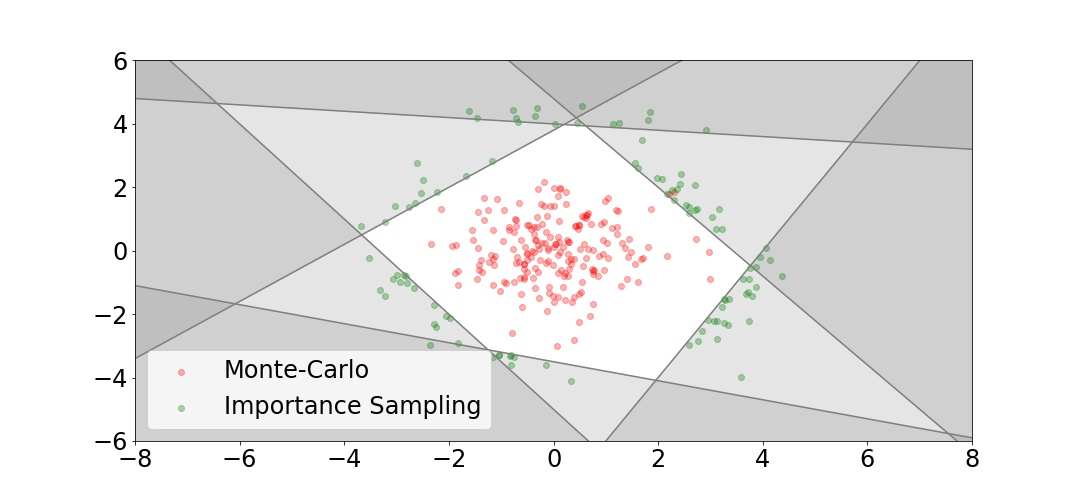
\includegraphics[width=.65\textwidth]{Dissertation/images/sampling/conditioned_vs_MC.jpg}
%     % \vspace{-5mm}
%     \caption{White area stands for generations that do not exceed operating limits. A set of generations leading to at least one constraint violation is in grey. Two or more reliability constraints are not satisfied in dark grey area. Samples from a nominal distribution and the constructed mixture marked in red and green resp. 
%     }
%     \label{fig:00}
%     % \vspace{-5mm}
% \end{figure}

% The estimate is estimated as \begin{align}\label{eq:aloe}
%     {\hat \Pi} = N^{-1}\sum_{i=1}^N \upsilon(p^i)/\upsilon_D(p^i, x^i), \quad p^i \sim D^{x^i},
% \end{align}
% where a distribution mixture $\{D_i\}_{i=1}^K$. The weights $\{x_i\}_{i=1}^K$ define the components of $D$, $p \sim \mathcal{N}(\mu, \Sigma)$ s.t. $p\not\in P$. The main idea is to find weights $x$ such that the estimate has the least variance. The iterative estimation process with updating weights $x^t_i, ~ i=1,\dots K, t=1, \dots k$ is given by
% \begin{align}
%     \hat \Pi = \frac{1}{k}\sum_{t=1}^k \frac{\upsilon(p^t) f(p^t)}{\upsilon_D(p^t, x^t)}, \; p^t \sim \upsilon_D(\cdot, x^t), t\le k \label{eq:emp}
% \end{align}

The last part of the section defines the optimization problem of finding a minimum of the estimate's variance and proves that the problem is convex in mixture weights $x_i$.
The variance minimization problem is
\begin{align}
    \min_x \; & V(x), \; 
    \text{s.t. } x_1 + \dots + x_K = 1, x_k \ge 0, 1\!\le\! k \!\le\! K\label{eq:var-min}
\end{align}
in $x$ for the mixture distribution $\upsilon_D(p,x) = \sum_{i=1}^K x_i \upsilon_i(p)$. %To improve numerical stability one may also add constraints $x_i \ge \varepsilon > 0$ that guarantee that the variance is bounded.
The section concludes with several theorems that establish the convexity of Problem \eqref{eq:var-min}, expression for its gradient, unbiasedness of the resulting estimate and expression for the estimate's variance.
% \begin{theorem}\label{thm:var-convexity}
% Problem~\eqref{eq:var-min} is convex in $x$, and for $x > 0$
% \begin{align*}
%     \nabla V(x) = \int_{\mathbb{R}^n} - f^2 (p)\upsilon^2(p)\upsilon_D^{-2}(p,x) (\upsilon_1(p), \dots, \upsilon_K(p))^\top dp.
% \end{align*} 
% \end{theorem}

% Importantly, the estimation studied is convex: 
% \begin{theorem}\label{thm:unbias}
% $\hat \Pi$ is an unbiased estimate of $\Pi$ if for all $k$, $1\le k \le N$, $x_k > 0$ and $x_k$ is independent of $x^j$ and $p^j$ for~$N\ge j > k\ge 1$.
% \end{theorem}

% Moreover, the variance of $\hat{\Pi}$ is also has the following property:
% \begin{theorem}\label{thm:var}
% Variance of $\hat\Pi$ equals $N^{-2}\sum_{k=1}^N V(x^k)$ if for all $k$ and $j,$ $1\le k < j \le N$, $x_k > 0$ and $x_k$ is independent of $x^j$ and~$p^j$.
% \end{theorem}

Section 3.3 setups the iterative scheme for updating weights $x^t$ using Mirror Descent with Bregman divergence based on negative entropy. The update is:
% \begin{align}\label{eq:md-upd}
%     \!\!x^{k+1} = \argmin\limits_{x\in S}\left\{\eta^k \nabla V(x^k)^\top (x - x^k) + D_\omega(x, x^k)\right\}\!\!,
% \end{align}
% where $S =\{x \ge 0,x_1+\dots+ x_K = 1\}$, a step-size $\eta^k \!>\! 0$, 
% $D_\omega(x, x^k)$ is the Bregman divergence defined for any strongly convex and smooth (distance-generating) function~$\omega$~as
% $
%     D_\omega(x, x^k) = \omega(x) - \{\omega(x^k) + \nabla \omega(x^k)^\top (x^k - x)\}.
% $
% So as the distance generating function is strongly convex and smooth in $x,$ so is the Bregman divergence. When $\omega(x) = \|x\|_2^2/2,$ mirror descent step is the same as in the gradient descent method, $x^{k+1} = x_k - \eta^k \nabla V(x^k)$. However, the negative entropy, $\omega(x) = -\sum_{i=1}^n x_i \log x_i$, is known to be the optimal choice for simplex constrained optimization. For $k\ge 1$ and $1\le i \le K$, solving~Eq.~\eqref{eq:md-upd} in $x$ leads to an update 
\begin{align}
\label{eq:_upd}x^{k+1}_i = x^k_i \frac{\exp(-\eta^k(\nabla V(x^k))_i)}{\sum_{j=1}^K x^k_j \exp(-\eta^k(\nabla V(x^k))_j)}, \eta^k > 0.
\end{align}

Next, the section presents the convergence properties
% \begin{theorem}\label{thm:lan}
%     For any function $V(x)$ that is $M$-Lipschitz in $\ell_1$ norm, i.e. $\|V(x) - V(y)\|_\infty \le M \|x-y\|_1 \forall x,y$, a constant step-size policy $\eta^k = \eta \le 1/M$, and 
%     a sequence $\{x^k\}_{k\ge 1}$ generated by \eqref{eq:md-upd} with $\omega(x) = \sum_{i\le K} x_i\log x_i$, one has
%     \begin{align*}
%         N^{-1}\sum_{i=1}^N (V(x^i)  - V^*) \le 
%         (\log K + (M^2 + \sigma^2) N \eta^2)/(N\eta),
%     \end{align*}
% with $\mathbb{E}_{\upsilon_D}\|g(p,x)- \nabla V(x)\|_\infty^2 \le \sigma^2$, $V_*$ is the optimum of~\eqref{eq:var-min}. 
% \end{theorem}
% To this end, according to Theorem~\ref{thm:lan} 
with the optimal choice of 
$\eta = M^{-1}\sqrt{\log K/(5N)},$ which yields almost dimension independent convergence rate stated in  Theorem~\ref{thm:md-c}. 
\begin{theorem}\label{thm:md-c} Mirror descent with an update~\eqref{eq:_upd} and a step-size policy $\eta^k \!=\! \eta M^{-1}\!\sqrt{(\log K)/N}$,  $\eta \sqrt{(\log K)/N}\!\le\! 1$ yields
\begin{align*}
    \mathbb{V}_{\upsilon_D} (\hat \Pi) = N^{-1}\sum_{k=1}^N V(x^k) < \frac{V^*}{N} +  \left(\frac{M}{\eta}+ \frac{5\eta}{M}\right)\frac{\sqrt{\log K}}{\eta N^{3/2}}, 
\end{align*}
with $M \!= \!\max_{i\le K}\varepsilon^{-2}\Pi_i^2$,  $x\!\ge\! \varepsilon$, $V^*$ be the optimum of~\eqref{eq:var-min}.
\end{theorem}

Compared to the earlier results of~\cite{owen2019importance}, the rate of convergence depends as $O(\sqrt{\log K})$ on the dimension $K$, while earlier results \cite{owen2019importance} claim linear dependence. Thus, the proposed methods results in a substantial acceleration for large-scale problems.

Section 3.4 presents an extensive numerical comparison of the proposed method with state-of-the-art estimation algorithms for the Gaussian polyhedron volume: pmvnorm and ALOE. The most important empirical findings are that there are two simple cases where pmvnorm and ALOE fail. The first one is a degenerate polytope and the second one is just a simple regular polytope with 360 faces that approximates a circle. Both cases are 2 dimensional.

% We consider a regular 2 dimensional polytope with $K$ faces ($K\ge 3$) centered at zero, $
%     P = \{p \in \mathbb{R}^2: \omega_j^\top x \leq \tau, 1\le j \le K\},
% $
% where $\omega_j = (\sin(2\pi j/K), \cos(2 \pi j/K))$. 
% We assume $p\sim\mathcal{N}(0, I_2)$, where $I_2$ is $2\times 2$ identity matrix. The probability $p\not\in P$ rapidly converges to $\exp(-\tau^2/2)$ as $K\to\infty$ \cite{owen2019importance}

% As the second example we consider a degenerate polytope with $K=1500$ faces, where $\omega_1 = (0, 1)$  and $\omega_j = (\xi, -1 - \xi)$, $2\le j \le K$. We take $\xi \sim \mathcal{U}[-\varepsilon, \varepsilon]$ for small $\varepsilon = 10^{-6}$. Note that $\omega_j$ for $j\geq 2$ are almost identical. Hence probability $\Pi$ is quite close to $2\Phi(-\tau)$.
% The results are shown in Figure \ref{fig:01}, showing stability of the proposed algorithm (MD-Var)

% \begin{figure}[t!]
%     \centering
%     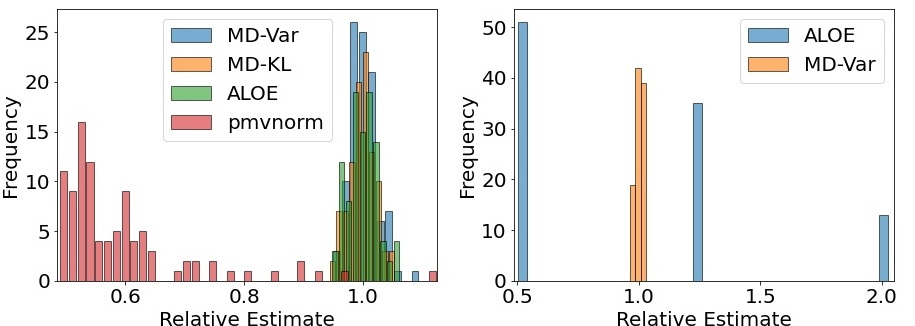
\includegraphics[width=.65\textwidth]{Dissertation/images/sampling/histograms.jpg}
%     %\vspace{-.5mm}
%     %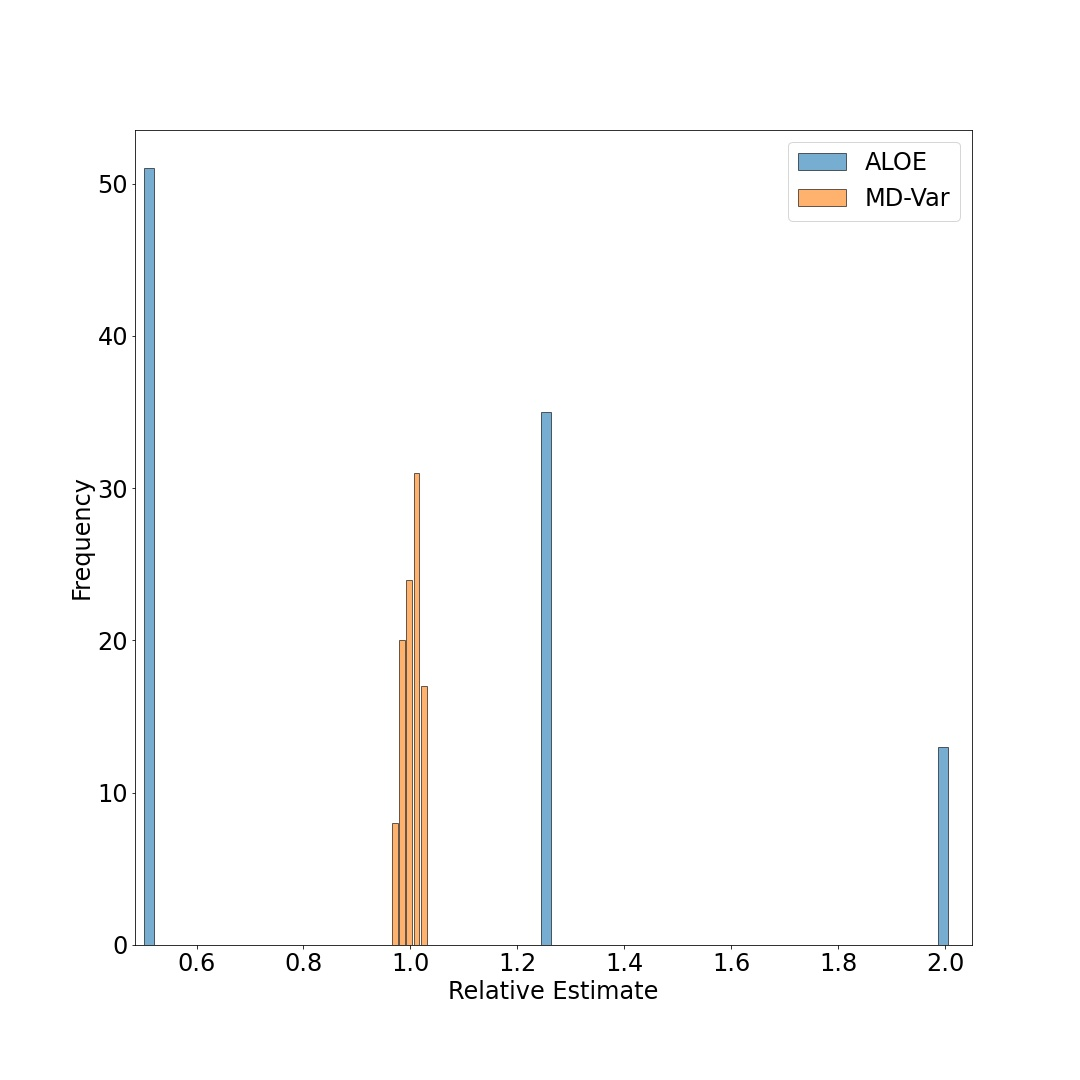
\includegraphics[width=.22\textwidth]{Dissertation/images/sampling/histogram_degenerate.jpg}%\hspace{-3mm}
%     %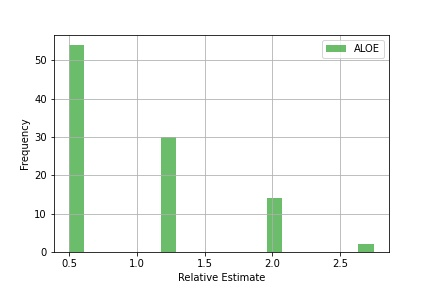
\includegraphics[width=.25\textwidth]{Dissertation/images/sampling/IS_hists_shivering_only_OMC.jpg}
%     \caption{Importance 
%     sampling methods performance on a 2-dimensional (left) regular polytope with $360$ faces; (right) degenerate polytope with $1500$ faces. Overload probabilities are  $\Phi(-6)$ and $2\Phi(-1)$ resp. 
%     }
%     \label{fig:01}
%     % \vspace{-5mm}
% %\end{figure}
% %\begin{figure}[t!]
% %    \centering
%     %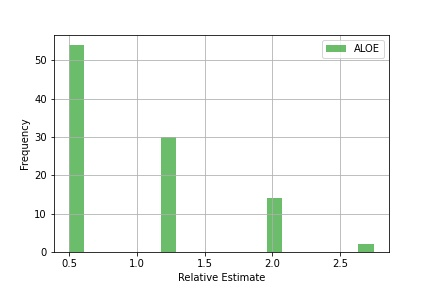
\includegraphics[width=.25\textwidth]{Dissertation/images/sampling/IS_hists_shivering_only_OMC.jpg}
%     %\caption{Importance 
%     %sampling methods performance on a 2-dimensional degenerate polytope with $1500$ faces and overload probability $2\Phi(-1)$.}
%     %\label{fig:degenerate_polytope}
%     %\vspace{-5mm}
% \end{figure}


For power grid test cases, we ran the algorithms on all the test cases accessible through PandaPower~\cite{pandapower.2018}. There were 27 cases with the number of buses varying from 4 to 9241. The proposed methods (MD-Var and MD-KL) took less than two minutes of computational time on a personal laptop for each of them. 
%
Table~\ref{tab:sample-compX} shows the minimal number of samples that are required by the algorithms to achieve \begin{align}    
\Pi/2 \le \hat\Pi \pm s(\hat\Pi) \le 3\Pi/2, \label{eq:tk}\end{align}
where $s(\hat\Pi)$ is the empirical standard deviation of the estimate. This ensures that not only the estimated value, but also its confidence interval is contained in $(\Pi/2, 3\Pi/2)$ and that the sum of the empirical estimate and its standard deviation are close to %of the same order as 
the true probability. 


\begin{table}[ht]
\centering
%\vspace{-4mm}
% \captionsetup{justification=centering}
\caption{Number of samples to satisfy Ineq.~\eqref{eq:tk} 
 for Iceland118}
 \begin{tabular}{|c|c|c|c|c|} 
 \hspace{-2mm}Bound ${\bar\theta}_{ij}$, probability $\Pi$ & MC & ALOE & Pmvnorm & MD-Var\\
 % &&& \cite{genz2020package} & (Section \ref{sampling:nm})\\
 \hline
  \hspace{-2mm}$|{\theta}_{ij}| \le \pi/8$, $\Pi$ = 1.2e-01 & 6.4e+02 & 3.7e+02 & \underline{3.2e+02} & 4.1e+02\\
  \hspace{-2mm}$|{\theta}_{ij}| \le \pi/7$, $\Pi$ = 3.0e-02 & 5.1e+04 & 4.1e+02 & 1.1e+03 & \underline{3.5e+02}\\
  \hspace{-2mm}$|{\theta}_{ij}| \le \pi/6$, $\Pi$ = 2.5e-03  & 6.2e+06 & 4.5e+02 & 6.3e+03 & \underline{3.9e+02} \\
  \hspace{-2mm}$|{\theta}_{ij}| \le \pi/5$, $\Pi$ = 2.6e-05  & 8.9e+10 & 3.3e+02 & 1.4e+04 & \underline{2.1e+02}\\
  \bottomrule
 \end{tabular}
 \vspace{-0mm}\label{tab:sample-compX}
\end{table}


% Table~\ref{tab:emp} shows overload probability estimates and their standard deviations for the algorithms based on $N = 200$ samples on various PandaPower~\cite{pandapower.2018} power grids.


Finally, the chapter concludes. Importance sampling proves invaluable for promptly evaluating the reliability of power grids in real-time scenarios. Our proposed algorithm innovatively creates a mixture distribution tailored to the grid's physics, enhancing accuracy. Through convex optimization, we fine-tune the mixture weights, surpassing existing methods in both precision and speed. This advancement opens doors for its application in optimizing and controlling power grids, promising enhanced efficiency and reliability.

\textbf{The fourth chapter} presents the approach for constructing scenario approximation for DC-OPF assuming additive Gaussian noise for generators. In other words, for linear program with additive Gaussian noise. 

The chapter starts with an introduction in Section 4.1 underscoring the industry need for efficient data-driven SA of Joint Chance Constrained (JCC) optimization problems for modeling optimal, reliable and non conservative generation regimes for high voltage power grids. 
%Next, this Section discusses recent advantages in this field and outlines the main problem: current ways of constructing SA are lead to extremely large linear optimization problems which are challenging to solve. Finally, it outlines the proposed solution - construct a proxy for redundant set of scenario and sample data using ALOE algorithm outside of that region.

Section 4.2 introduces notation and recalls the polyhedron in generation vector $p$ as in Chapter 3. Next, it formulates the JCC optimization problem under consideration:
\begin{equation}\label{eq:JCC-OPF}
    \begin{aligned}
  \min_x & \;\mathbb{E}_{\xi\sim \mathcal{N}(0, \Sigma)} \textit{cost}(x,\xi)\\
   \textit{s. t. }\; & \mathbb{P}_{\xi\sim \mathcal{N}(0, \Sigma)} (x+\xi \in \mathcal{P}) \ge 1 - \eta
   \end{aligned}
\end{equation}

Finally, it presents the SA for this JCC and recalls the number of data samples required to obtain $1-\delta$ reliable solution, i.e., solution of SA that is feasible to original JCC with probability $1-\delta$:
\begin{align}\label{eq:sc-opf}
  \min_x & \; \frac{1}{N} \sum_{t=1}^N \textit{cost}(x,\xi^t)\\
  \textit{s. t. } & \; p^{\min} \le x+\xi^t \le p^{\max}, \; 1\le t \le N\nonumber\\
  & \; |\theta_i(\xi^t) - \theta_j(\xi^t)| \le {\bar \theta}_{ij}, (i, j)\in \mathcal{E}, \; 1\le t \le N\nonumber\\
  & x+\xi^t = B \theta(\xi^t), \; 1\le t \le N\nonumber
\end{align}
The key disadvantage of the scenario approximation \eqref{eq:sc-opf} is the number of constraints induced by adding scenarios $\xi^t$. A classical theory, developed by Calafiore and Campi \cite{calafiore2006scenario}, suggests to include a large number of scenarios $N$. This will allow the solution of \eqref{eq:sc-opf} to be feasible for original problem \eqref{eq:JCC-OPF} with high probability $1 - \delta$. However, the number of required scenarios $N$ is given by $N \geq 2 \left( \frac{\ln{1/\delta}}{\eta} + d + d\frac{\ln{1/\eta}}{\eta} \right)$, where $d$ is the number of control variable in the optimization problem. For example, with $\eta = 10^{-2}, \delta = 10^{-2}$, for  IEEE-57 case one would end up with $6.45 \cdot 10^3$ (6 generators, excluding slack one) constraints which is time- and memory-consuming to solve.

Section 4.3 present the sketch of the proposed approach, formalizes it introduces the redundant region, applies importance sampling. Finally, it presents the theorems that prove the theoretical advantage in number of scenarios in SA.

It starts with the discussion of interrelations between original deterministic feasibility set under probability $\mathcal{P}$, and approximations of JCC feasibility sets. 

The approach follows these steps:

\begin{enumerate}
    \item Construct an inner approximation of the feasibility set.
    \item Generate samples outside this approximation.
    \item Solve the scenario approximation Problem using the generated samples.
\end{enumerate}


First, leveraging the fact that "the probability of a union of events is bounded from below by the maximum of individual event probabilities," we establish a lower bound on the probability of constraint feasibility $\mathbb{P}(x+\xi \in \mathcal{P})$. This allows us to add constraints $x\in \mathcal{P}_{out}$, ensuring that if $x \notin \mathcal{P}_{out}$, then $\mathbb{P}(x+\xi \notin \mathcal{P}) > \eta$. Hence, if the solution $\bar x$ of the scenario approximation with samples from the nominal distribution $\mathcal{N}(0,\Sigma)$ satisfies $\mathbb{P}(x+\xi \in \mathcal{P}) \ge 1-\eta$, adding constraints $x \in \mathcal{P}_{out}$ does not alter $\bar x$.

Second, using the aforementioned bound, we define a polytope $\mathcal{P}{\texttt{in}}(x) = {p: W_{\texttt{in}} \xi \le b_{\texttt{in}}, p = x+\xi}$ around $x$, with $W_{\texttt{in}}$ and $b_{\texttt{in}}$ independent of $x$, which is illustrated in Figure~\ref{fig:10}
%The exact expressions for $W_{\texttt{in}}$ and $b_{\texttt{in}}$ are given in Theorem \ref{thm:20} and illustrated in Figure~\ref{fig:10}.

We demonstrate that for any sample $\xi^t$ and feasible $x$, if $p = x+\xi^t \in \mathcal{P}_{\texttt{in}}(x)$, then $p$ also belongs to the constraint feasibility set $\mathcal{P}$. Thus, scenarios $\xi^t: x+\xi^t \in \mathcal{P}_{\texttt{in}}$ can be excluded from the SA optimization problem  without losing approximation accuracy.

Finally, we sample scenarios outside of the polyhedron $\mathcal{P}_{\texttt{in}}$ using state-of-the-art importance sampling methods \cite{owen2019importance,lukashevich2021power} and solve the Scenario Approximation Problem with the generated samples.
\def\shift{2.7}
\def\shiftt{2.35}
\def\shiftuselesssample{0.3}
\def\shiftusefulsample{1.1}
\begin{figure}
    \centering
        \begin{tikzpicture}[scale=0.75, node distance={15mm}, thick, main/.style = {draw, scale=.9}] 
        %x
        \coordinate (x) at (0, 0);
        \draw (x) circle (1pt);
        \draw (x) ++(0.05, 0.05) node[above right] (tmp) {$x$};
        %x2
        \coordinate (x2) at (0 + \shiftt, 0 - \shiftt);
        \draw (x2) circle (1pt);
        \draw (x2) ++(0.05, 0.05) node[above right] (tmp) {$x^*$};
        %outer guy
        \coordinate (a) at ( 4.755282581475767 , 1.545084971874737 );
        \coordinate (b) at ( 3.061616997868383e-16 , 5.0 );
        \coordinate (c) at ( -4.755282581475767 , 1.5450849718747375 );
        \coordinate (d) at ( -2.9389262614623664 , -4.045084971874736 );
        \coordinate (e) at ( 2.9389262614623646 , -4.045084971874738 );
        %linking outer guy
        \draw (a) -- (b);
        \draw (b) -- (c);
        \draw (c) -- (d);
        \draw (d) -- (e);
        \draw (e) -- (a);
        %annotating outer guy
        \draw
        (a) ++(0.1, 0.01) node[above] (tmp) {$\mathcal{P}$};
        %(tmp.west) -- (PO);
        
        %green guy
        \coordinate (ag) at ( 3.804226065180614 , 1.2360679774997896 );
        \coordinate (bg) at ( 2.4492935982947064e-16 , 4.0 );
        \coordinate (cg) at ( -3.804226065180614 , 1.23606797749979 );
        \coordinate (dg) at ( -2.351141009169893 , -3.2360679774997894 );
        \coordinate (eg) at ( 2.3511410091698917 , -3.2360679774997902 );
        %linking green guy
        \draw [olive] (ag) -- (bg);
        \draw [olive] (bg) -- (cg);
        \draw [olive] (cg) -- (dg);
        \draw [olive] (dg) -- (eg);
        \draw [olive] (eg) -- (ag);
        %annotating green guy
        \draw
        (bg) ++(0.1, 0.01) node[below, olive] (tmp) {$\mathcal{P}_{out}$};
        %(tmp.west) -- (PO);
        
        %red guy
        \coordinate (ar) at ( 0.9510565162951535 , 0.3090169943749474 );
        \coordinate (br) at ( 6.123233995736766e-17 , 1.0 );
        \coordinate (cr) at ( -0.9510565162951535 , 0.3090169943749475 );
        \coordinate (dr) at ( -0.5877852522924732 , -0.8090169943749473 );
        \coordinate (er) at ( 0.5877852522924729 , -0.8090169943749476 );
        %linking red guy
        \draw [red] (ar) -- (br);
        \draw [red] (br) -- (cr);
        \draw [red] (cr) -- (dr);
        \draw [red] (dr) -- (er);
        \draw [red] (er) -- (ar);
        %annotating red guy
        \draw
        (br) ++(1em, .1em) node[above right, red] (tmp) {$\mathcal{P}_{\texttt{in}}(x)$};
        %(tmp.west) -- (PO);
        
        %red guy2
        \coordinate (ar2) at ( 0.9510565162951535 + \shiftt , 0.3090169943749474 - \shiftt);
        \coordinate (br2) at ( 6.123233995736766e-17 + \shiftt , 1.0  - \shiftt);
        \coordinate (cr2) at ( -0.9510565162951535  + \shiftt, 0.3090169943749475  - \shiftt);
        \coordinate (dr2) at ( -0.5877852522924732 + \shiftt, -0.8090169943749473 - \shiftt);
        \coordinate (er2) at ( 0.5877852522924729 + \shiftt, -0.8090169943749476  - \shiftt);
        %linking red guy
        \draw [red] (ar2) -- (br2);
        \draw [red] (br2) -- (cr2);
        \draw [red] (cr2) -- (dr2);
        \draw [red] (dr2) -- (er2);
        \draw [red] (er2) -- (ar2);
        %annotating red guy
        \draw
        (br2) ++(1em, .1em) node[above, red] (tmp) {$\mathcal{P}_{\texttt{in}}(x^*)$};
        %(tmp.west) -- (PO);
        
        %Upper \Delta_i
        \coordinate (b_) at (1, 5.7265);
        \draw
        (b_) node[above right] (tmp) {$\Delta_i$};
        %(tmp.west) -- (PO);
        \coordinate (bg_) at (1.5, 5.0898);
        \draw [dashed] (b) -- (b_);
        \draw [dashed] (bg) -- (bg_);
        \draw [thick, black, -latex'] (b_) -- (bg_);
        \draw [thick, black, -latex'] (bg_) -- (b_);
        
        %Inner \Delta_i
        \coordinate (br_) at (-1.5, -0.0898137920080413);
        \draw
        (br_) node[above left] (tmp) {$\Delta_i$};
        %(tmp.west) -- (PO);
        \coordinate (x0_) at (-1.0, -0.7265425280053608);%x!
        \draw [dashed] (br) -- (br_);
        \draw [dashed] (x) -- (x0_);
        \draw [thick, black, -latex'] (br_) -- (x0_);
        \draw [thick, black, -latex'] (x0_) -- (br_);
        
        %Inner \Delta_i 2
        \coordinate (br_2) at (-1.5 + \shiftt, -0.0898137920080413 - \shiftt);
        \draw
        (br_2) node[above left] (tmp) {$\Delta_i$};
        %(tmp.west) -- (PO);
        \coordinate (x0_2) at (-1.0 + \shiftt, -0.7265425280053608-  \shiftt);%x!
        \draw [dashed] (br2) -- (br_2);
        \draw [dashed] (x2) -- (x0_2);
        \draw [thick, black, -latex'] (br_2) -- (x0_2);
        \draw [thick, black, -latex'] (x0_2) -- (br_2);
        
        % Samples
        %% Useless
        \coordinate (xu_1) at (\shiftt + \shiftusefulsample * 0.1, -\shiftt - 3.5*\shiftuselesssample);
        \draw [teal] (xu_1) circle (1pt);
        \coordinate (xu_2) at (\shiftt + \shiftusefulsample, -\shiftt + \shiftusefulsample * 0.5);
        \draw [teal] (xu_2) circle (1pt);
        \coordinate (xu_3) at (\shiftt - \shiftusefulsample * 0.2, -\shiftt + \shiftusefulsample);
        \draw [teal] (xu_3) circle (1pt);
        \coordinate (xu_4) at (\shiftt + \shiftusefulsample * 0.7, -\shiftt - \shiftusefulsample);
        \draw [teal] (xu_4) circle (1pt);
        \end{tikzpicture}  
\caption{We consider a deterministic feasibility set $\mathcal{P}$ and derive a polytope $\mathcal{P}_{out}$ inside of it so that no optimal solution $x^*$ of Prob.~ \eqref{eq:JCC-OPF} belongs to $\mathcal{P}\setminus \mathcal{P}_{out}$. The polytope $\mathcal{P}_{\texttt{in}}(x)$ depicts the distances between the planes of $\mathcal{P}$ and $\mathcal{P}_{out}$ for each $x$.
%The polytope $\mathcal{P}_{\texttt{in}}$, defined in terms of noise $\xi$ only, $.
Samples of uncertainty outside $\mathcal{P}_{\texttt{in}}(0)$ are used to determine optimal solution using importance sampling.}
  \label{fig:10}
  %\vspace
\end{figure}

The inner approximation can be obtained by the Boole-Frechet inequality:
\begin{align*}
  \mathbb{P}&(p\in \mathcal{P}) = 
  \mathbb{P}(p: Wp \le b) =\\
  & 1 - \max_{1\le i\le J}\mathbb{P}\left(p: \omega_i^\top p > b_i\right).
\end{align*}
Further, taking into account Gaussianity and considering the case when there exists a plane that exceed the probability $\eta$, one can obtain the following expression for the outer approximation of the JCC - $\mathcal{P}_{out}$:

\begin{align}\label{eq:05}
  P_{out} = \left\{x: \omega_i^\top x \le b_i - \Delta_i, 1\leq i\leq J\right\},
\end{align}

where $\Delta_i = \|\Sigma^{1/2}\omega_i\|_2 \Phi^{-1}(1-\eta)$, $\eta \le 1/2$.

% For this outer JCC approximation set an important theorem is stated and proved. This theorem proves that the outer approximation is also satisfied for a solution of original JCC problem:
% \begin{theorem}\label{thm:10}
%   The joint chance-constrained optimal power flow problem~ \eqref{eq:JCC-OPF} has the same set of optimal solutions as 
%   \begin{align}\label{eq:JCC-OPF-Ad}
%   \min_x & \;\mathbb{E}_{\xi\sim \mathcal{N}(0, \Sigma)} \textit{cost}(x,\xi)\\
%    \textit{s. t. }\; & \mathbb{P}_{\xi\sim \mathcal{N}(0, \Sigma)} (x+\xi \in \mathcal{P}) \ge 1 - \eta, 0 < \eta \le 1/2,\nonumber\\
%    & \; x\in \mathcal{P}_{out}\nonumber 
% \end{align}
% \end{theorem}

% It is also important to prove that for the SA without including $\mathcal{P}_{out}$ the same logic applies:
% \begin{theorem}\label{thm:20}
% Any solution of the Scenario approximation problem~ \eqref{eq:sc-opf} that is feasible for the Chance-constrained OPF problem~ \eqref{eq:JCC-OPF} is also a solution of 
% %\newpage
% %\begin{align}\label{eq:30}
The Scenario Approximation is given as
\begin{subequations}
\label{eq:Fin}
  \begin{equation}
  \min_x \; \textit{cost}(x)\nonumber
  \end{equation}
  \begin{equation}
  \hspace{-20mm}\textit{s. t. }\;\; p^{\min} \le x+\xi^t \le p^{\max}, \; 1\le t \le N\label{eq:Fin-a}
  \end{equation}
  \begin{equation}
   \hspace{11mm} |\theta_i(\xi^t) - \theta_j(\xi^t)| \le {\bar \theta}_{ij}, (i, j)\in \mathcal{E}, \; 1\le t \le N\label{eq:Fin-b}
  \end{equation}
  \begin{equation}
  \hspace{-19mm} x+\xi^t = B \theta(\xi^t), \; 1\le t \le N\label{eq:Fin-c}
  \end{equation}
  \begin{equation}
  \hspace{-50mm} x\in \mathcal{P}_{out} \label{eq:Fin-d}
  \end{equation}
\end{subequations} 
% \end{theorem}

Recall the standard fundamental assumption that ensures the correctness of theorems that state the lower bound for required number of scenarios from~\cite{calafiore2006scenario}:
\begin{assumption}\label{asmp:10}
Assume that for all possible uncertainty realizations $\xi^1, \dots, \xi^N$, the optimization problem \eqref{eq:Fin} is either infeasible or, if feasible, it attains a unique optimal solution.
\end{assumption}

This assumption allows to proof the main theorem of this chapter. The following statement shows that the number of scenarios required is reduced by the measure of $\mathcal{P}_{in}$ which is denoted by $\pi$:
\begin{theorem}\label{thm:40}
Let $\bar x_N$ be a unique solution of the Scenario optimization Problem~\eqref{eq:Fin} with $N$ i.i.d. samples, so that none of the samples belong to $\mathcal{P}_{\texttt{in}}$. Moreover, assume that for any $N$ the assumption \ref{asmp:10} is fulfilled. Then for any $\delta \in (0,1)$ and any~$\eta \in (0, 1/2]$, $\bar x_N$ is also a solution for the Chance-constrained optimal power flow Problem~\eqref{eq:JCC-OPF} with probability at least $1-\delta$ if 
\begin{align*}
  N \ge \left\lceil 2\frac{(1-\pi)\ln \frac{1}{\delta}}{\eta} + 2d + 2d (1-\pi) \frac{\ln\frac{2(1-\pi)}{\eta}}{\eta} \right\rceil, 
\end{align*} 
where $d$ is a dimension of the space of controllable generators, and $\pi$ is the probability of a random scenario $\xi\sim \mathcal{N}(0, \Sigma)$ to belong to $\mathcal{P}_{\texttt{in}}$, and $\pi < 1$. 
\end{theorem}

Unfortunately, there isn't a precise and efficient algorithm for sampling from a Gaussian distribution outside a convex polytope \cite{khachiyan1993complexity}. However, the ALOE algorithm \cite{owen2019importance, lukashevich2021power} provides a sophisticated method for approximating the desired distribution by sampling from a mixture of distributions.

We focus on Gaussian fluctuations of power injections, $\xi \sim \mathcal{N}(0, \Sigma)$, with known covariance matrix $\Sigma \in \mathbb{R}^{n \times n}$. Our aim is to sample scenarios outside $\mathcal{P}_{\texttt{in}}$, ensuring that the sampling distribution closely approximates the conditional Gaussian distribution $\xi \sim \mathcal{N}(0, \Sigma) \textit{s.t. } \xi \not\in \mathcal{P}_{\texttt{in}}$.

We use the same algorithm for sampling from distribution $D$ as in previous chapter:
\begin{align}\label{eq:q_d}
  D = \sum_{i=1}^J \alpha_i D_i, \; & \alpha_i \ge 0, \sum_{i=1}^J \alpha_i = 1,\nonumber \\
  & \alpha_i \propto \Phi(-\Delta_i/\|\Sigma^{1/2}\omega_i\|_2),
\end{align}
where $\Phi$ is a CDF of the standard normal distribution. Let $q_D(\xi)$ be a PDF of distribution $D$, then Theorem~\ref{thm:50} established a maximal ratio of the conditional Gaussian density~$\xi\sim\mathcal{N}(0, \Sigma) \textit{s. t. } \xi\not\in\mathcal{P}_{\texttt{in}}$ and~$q_D(\xi)$.

It is important to formalize the inaccuracy of modeling the Gaussian conditioned on a polyhedron's complement with out-of-plane Gaussian mixtures.
Let $q_D(\xi)$ be a PDF of distribution $D$, then Theorem~\ref{thm:50} established a maximal ratio of the conditional Gaussian density~$\xi\sim\mathcal{N}(0, \Sigma) \textit{s. t. } \xi\not\in\mathcal{P}_{\texttt{in}}$ and~$q_D(\xi)$. 

\begin{theorem}\label{thm:50}
Let $\nu(\xi)$, $q_D(\xi)$ be PDFs  of $\xi\sim\mathcal{N}(0, \Sigma) \textit{s. t. } \xi\not\in\mathcal{P}_{\texttt{in}}$, and a mixture density (see Eq.~\eqref{eq:q_d}), resp. Then for any $\xi\not\in\mathcal{P}_{\texttt{in}}$, we have
\begin{align}\label{eq:M}
  \nu(\xi) \le M q_D(\xi),  
  M = \frac{\sum_{i\le J} \Phi(-\Delta_i/\|\Sigma^{1/2}\omega_i\|_2)
  }{\max_{i\le J}\Phi(-\Delta_i/\|\Sigma^{1/2}\omega_i\|_2)}, 
\end{align}
where $D$ and $\alpha_i$ are given in Eq.~\eqref{eq:q_d}.
\end{theorem}

In particular, we solve the following optimization problem instead of Problem~\eqref{eq:sc-opf}: 
\begin{subequations} 
\label{eq:FinA}
  \begin{equation}
  \min_x \; \textit{cost}(x)\nonumber
  \end{equation}
  \begin{equation}
  \hspace{-20mm}\textit{s. t. }\;\; p^{\min} \le x+\xi^t \le p^{\max}, \; 1\le t \le N\label{eq:FinA-a}
  \end{equation}
  \begin{equation}
   \hspace{11mm} |\theta_i(\xi^t) - \theta_j(\xi^t)| \le {\bar \theta}_{ij}, (i, j)\in \mathcal{E}, \; 1\le t \le N\label{eq:FinA-b}
  \end{equation}
  \begin{equation}
  \hspace{-19mm} x+\xi^t = B \theta(\xi^t), \; 1\le t \le N\label{eq:FinA-c}
  \end{equation}
  \begin{equation}
  \hspace{-50mm} x\in \mathcal{P}_{out} \label{eq:FinA-d}
  \end{equation}
  \begin{equation}
  \hspace{-32mm} \xi^1, \xi^2, \dots, \xi^N\sim D \label{eq:FinA-e},
  \end{equation}
\end{subequations}

Finishing the practical implementation, the next theorem shows the advantage in number of samples required to obtain reliable SA solution:

\begin{theorem}\label{thm:80}
Let $\bar x_N$ be a unique solution of the Scenario optimization Problem~\eqref{eq:FinA} with $N$ i.i.d. samples follow distribution $D$. Moreover, assume that for any $N$ the assumption \ref{asmp:10} is fulfilled. Then for any $\delta \in (0,1)$ and any~$\eta \in (0, 1/2]$, $\bar x_N$ is also a solution for the chance-constrained optimal power flow Problem~\eqref{eq:JCC-OPF} with probability at least $1-\delta$ if 
\begin{align*}
  N \ge \left\lceil 2M\frac{(1-\pi)\ln \frac{1}{\delta}}{\eta} + 2d + 2d M(1-\pi) \frac{\ln\frac{2M(1-\pi)}{\eta}}{\eta} \right\rceil, 
\end{align*} 
where $d$ is a dimension of the problem and $\pi$ is a probability of a random scenario $\xi$ to belong to $\mathcal{P}_{\texttt{in}}$, $\pi < 1$, and constant $M$ is defined by Theorem~\ref{thm:50}.
\end{theorem}

% The Section 5.4 presents the numerical comparison of the proposed approach with classical Monte-Carlo based SA. The core of this section is the experimental protocol. The methods are compared based on the estimated solution reliability $1-\hat{\delta}$, i.e., the probability that the SA's solution is feasible to the original JCC. The procedure is summarized in Algorithm \ref{alg:estimate_delta}.
% \begin{algorithm}[ht]
% \SetKwInOut{Input}{input}
% \SetKwRepeat{Do}{do}{while}
% % \SetKwInOut{Output}{output}
% \caption{Reliability $1-\hat{\delta}$ -- an empirical estimate}\label{alg:estimate_delta}
% \Input{$L$ -- number of trials, DC-OPF problem parameters, $\eta$ -- confidence level, $N_0$ -- initial size of scenario approximation, $N_{\max}$ -- maximal size of scenario approximation}
% $N \gets N_0$\;
% $\hat{ \boldsymbol \delta}$ -- storage for $\hat{\delta}_N$\;
% \Do{$N \leq N_{\max}$}
% {
%      $C_N \gets 0$ -- feasibility counter\;
%      $l \gets 1$\;
%     \Do{$l \leq L$}{
%         Obtain $(x^*_N)_l$ -- scenario approximation with $N$ samples (using SA-IS or SA) \;
%         Estimate constraint satisfaction probability $(\hat{\mathbb{P}}_N)_l$ using Monte Carlo samples.\; \label{alg:estimate_delta:phat_N_l}\;
%         \uIf{$(\hat{\mathbb{P}}_N)_l \geq 1 - \eta$}{
%             $C_N \gets C_N +1$
%         }
%         }
%     $1-\hat{\delta}_N \gets C_N / L$ -- fraction of trials turned out to be feasible \;
%     Append $\hat{\delta}_N$ to $\hat{ \boldsymbol \delta}$ \;
%     $n  \gets n + N_{\max}/ 10$\;
% }
% \Return $\hat{ \boldsymbol \delta}$
% \end{algorithm}

The results of comparison are presented in Table \ref{tab:summary_results}. Additionally, the reliability analysis of approximations' solutions is presented in Figures \ref{fig:spreads}, \ref{fig:empiricals}, the latter illustrates empirical reliability ($1-\hat{\delta}$) and the former illustrates the spread of constraint feasibility $(\hat{\mathbb{P}}_N)_l$ for CC-OPF ($1-\eta =.99$) for IEEE 300 bus and IEEE 118 bus systems. The three cases correspond to samples in CC-OPF being drawn by SA, SA-IS and SA-O. The empirical estimates are computed with $L = 100$ optimization instances (for $1-\hat{\delta}$), and $N_{MC}=10^4$ Monte-Carlo samples for each instance to determine constraint validation (for box-plot of $(\hat{\mathbb{P}}_N)_l$). 
Colored boxes stands for the 25\% -- 75\% interquantile range (IQR). Diamonds shows samples outside of the $\pm 1.5*\text{IQR}$. 
Note that both in reliability, and the IRQ of constraint feasibility, SA-IS requires much less number of samples compared to SA or~SA-O. Finally, the execution time of the preprocessing step comparison is visualized in Figure \ref{fig:profile_generate_samples}. On the right Figure, vertical dashed lines indicate number of samples that are sufficient to reach $1-\hat{\delta}=0.99$ reliability level for $\eta=0.05$, see Table \ref{tab:summary_results}. Horizontal dot-dashed lines demonstrate the amount of time spent on average over 15 runs. From this figure, one can observe that ALOE is a more time consuming procedure. However, one can observe that the time required to solve scenario approximations together with preprocessing does not differ significantly for IS-SA and SA -- see Figure \ref{fig:profile_scenario_approx}. The latter figure also shows that the computational time required to obtain the same reliability level is five times less for SA-IS (the number of samples are taken from Table \ref{tab:summary_results}, case IEEE-30, $\eta=0.05$.)

\begin{landscape}
\begin{table*}[t]
\caption{Number of SA-IS and SA samples required to reach reliability level $1-\hat{\delta} = 0.99$ in CC-OPF with confidence threshold $1-\eta$. The number of scenarios required for target reliability were obtained empirically, iterating over a predefined grid for $N$ with the step of $10$.
    The confidence threshold $1-\eta$ is estimated using Monte Carlo samples (out of sample) and empirical reliability is computed by averaging over $L=100$ independent CC-OPF problem instances. The costs of solutions obtained are depicted alongside with the corresponding costs of deterministic DC-OPF solution. It is clear that SA-IS requires much less samples compared to SA, while maintaning the same reliability of the solution.}
    \centering
        \begin{tabular}{|lrrll|rll|l|}
        \toprule
           Case &  $\eta$ &  SA No &  SA Cost &   SA $(\mathbb{P}_N)$ &  IS-SA No & IS-SA Cost & IS-SA $(\mathbb{P}_N)$ & DC-OPF Cost \\
        \midrule
         grid30 &    0.05 &    160 & 5.89e+03 & 9.82e-01$\pm$7.09e-03 &        \textbf{60} &   5.87e+03 &  9.80e-01$\pm$8.86e-03 &    5.67e+03 \\
         grid57 &    0.05 &    210 & 2.52e+04 & 9.78e-01$\pm$8.95e-03 &       \textbf{160} &   2.52e+04 &  9.89e-01$\pm$7.71e-03 &    2.50e+04 \\
        grid118 &    0.05 &   1300 & 8.72e+04 & 9.68e-01$\pm$4.18e-03 &      \textbf{1050} &   8.72e+04 &  9.68e-01$\pm$4.16e-03 &    8.48e+04 \\
        grid300 &    0.05 &   1550 & 4.72e+05 & 9.63e-01$\pm$4.36e-03 &      \textbf{1250} &   4.72e+05 &  9.62e-01$\pm$3.97e-03 &    4.71e+05 \\
        \midrule
         grid30 &    0.01 &    800 & 5.94e+03 & 9.96e-01$\pm$1.83e-03 &       \textbf{300} &   5.96e+03 &  9.99e-01$\pm$6.57e-04 &    5.67e+03 \\
         grid57 &    0.01 &   1300 & 2.52e+04 & 9.96e-01$\pm$1.55e-03 &       \textbf{300} &   2.53e+04 &  9.97e-01$\pm$1.88e-03 &    2.50e+04 \\
        grid118 &    0.01 &   6000 & 8.74e+04 & 9.93e-01$\pm$1.16e-03 &      \textbf{3600} &   8.74e+04 &  9.94e-01$\pm$9.11e-04 &    8.48e+04 \\
        grid300 &    0.01 &   9000 & 4.72e+05 & 9.93e-01$\pm$8.42e-04 &      \textbf{4500} &   4.72e+05 &  9.92e-01$\pm$9.53e-04 &    4.71e+05 \\
        \bottomrule
        \end{tabular}
    \label{tab:summary_results}
\end{table*}
\end{landscape}
\begin{figure*}[hbt]
\centering
\begin{subfigure}{.8\textwidth}
  \centering
  % include first image
  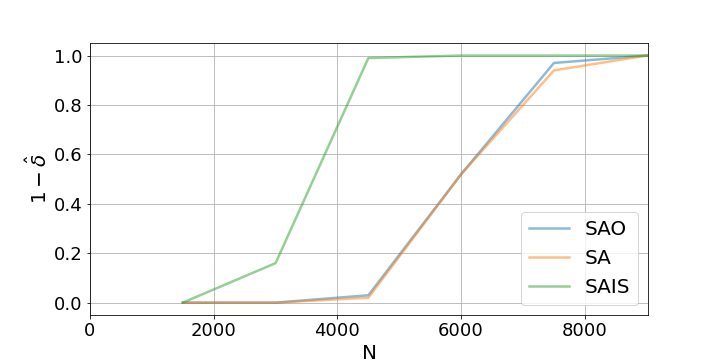
\includegraphics[width=0.99\linewidth]{Dissertation/images/dc_stochastic_approx/case300/1_beta_N_12000_eta_001.png}~~~~~~\hfill
  \caption{IEEE 300 bus system.}
  \label{fig:ieee300reliability}
\end{subfigure}

\begin{subfigure}{.8\textwidth}
  \centering
  % include first image
  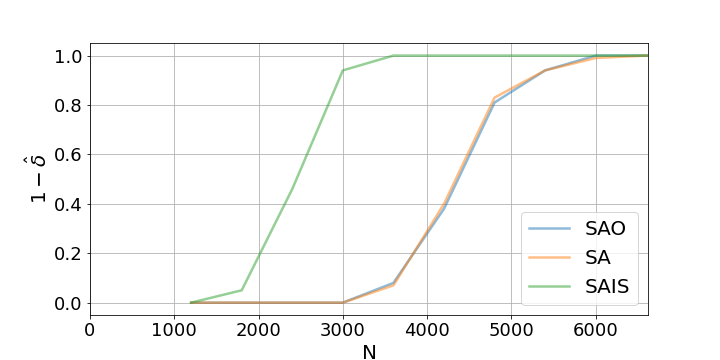
\includegraphics[width=0.99\linewidth]{Dissertation/images/dc_stochastic_approx/ieee118/1_beta_N_7800_eta_001.png}~~~~~~\hfill
  \caption{IEEE 118 bus system.}
  \label{fig:ieee118reliability}
\end{subfigure}
\caption{Empirical reliability ($1-\hat{\delta}$) versus number of samples in \\CC-OPF ($N$).}
\label{fig:empiricals}
\end{figure*}

\begin{figure*}[hbt]
\centering
\begin{subfigure}{.8\textwidth}
  \centering
  % include second image
  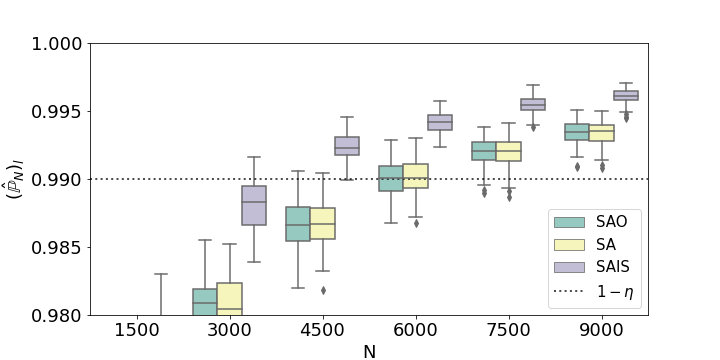
\includegraphics[width=0.99\linewidth]{Dissertation/images/dc_stochastic_approx/case300/boxplot_J_N_9000_eta_001.png}
  \caption{IEEE 300 bus system.}
  \label{fig:ieee300conservatism}
\end{subfigure}

\begin{subfigure}{.8\textwidth}
  \centering
  % include second image
  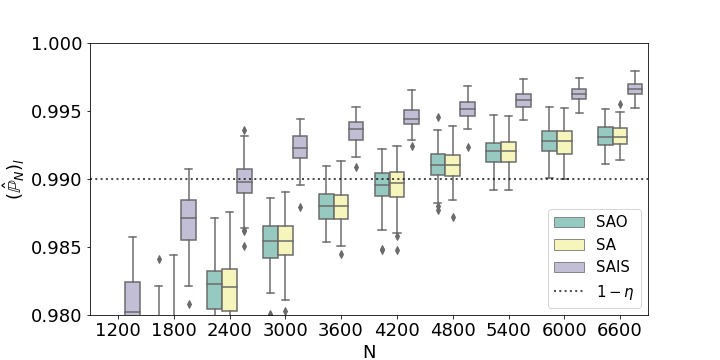
\includegraphics[width=0.99\linewidth]{Dissertation/images/dc_stochastic_approx/ieee118/boxplot_J_N_6600_eta_001.png}
  \caption{IEEE 118 bus system.}
  \label{fig:ieee118conservatism}
\end{subfigure}
\caption{Spread of probability of constraint feasibility ($(\hat{\mathbb{P}}_N)_l$) versus number of samples in CC-OPF ($N$).}
\label{fig:spreads}
\end{figure*}

\begin{figure*}[hbt]
\centering
\begin{subfigure}{.8\textwidth}
  \centering
  % include first image
  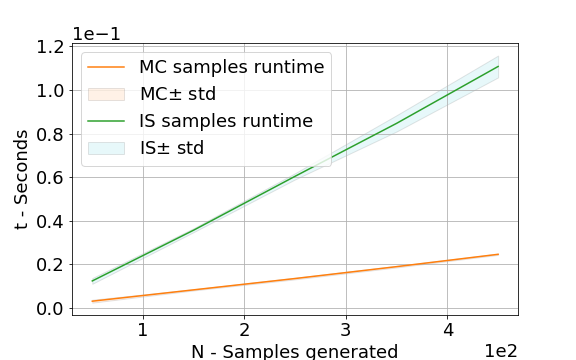
\includegraphics[width=0.9\linewidth]{Dissertation/images/dc_stochastic_approx/profiling_samplig.png}~~~~~~\hfill
  \caption{Sample generation.}
  \label{fig:profile_generate_samples}
\end{subfigure}
\begin{subfigure}{.8\textwidth}
  \centering
  % include second image
  \hspace{-10mm}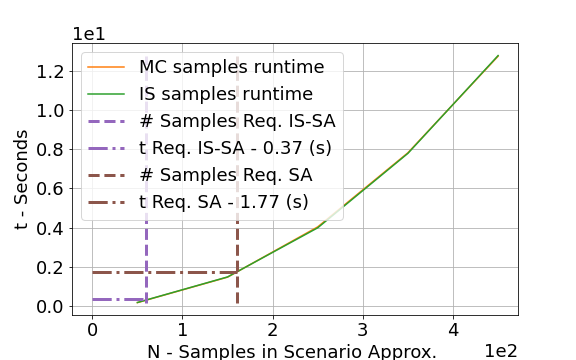
\includegraphics[width=0.9\linewidth]{Dissertation/images/dc_stochastic_approx/profiling_approx_sol.png}
  \caption{Samples preparation, assembling scenario approximation and solving the latter, formed for different $N$.}
  \label{fig:profile_scenario_approx}
\end{subfigure}
\caption{Computational time required to complete prepocessing step \ref{fig:profile_generate_samples} and solve corresponding scenario approximations \ref{fig:profile_scenario_approx} for IEEE-30 case. }
\label{fig:profiling}
\end{figure*}
The experiments were conducted on power system test cases and indicate the robustness and higher data efficiency of the proposed approach.

Finally, the Chapter concludes. In this chapter, we explored scenario approximation for chance-constrained optimal power flow, demonstrating that importance sampling enhances accuracy and reduces numerical complexity for stochastic OPF.
Our theoretical analysis highlights the advantages of using violative samples. Numerical experiments show a significant reduction in sample size needed for high reliability. This approach can also be extended to automated real-time control of bulk power systems.

\textbf{The fifth chapter} presents a generalization for power grid with dynamics. The whole approached as called A-priori Reduced Scenario Approximation (AR-SA). Here the uncertainty is a total power mismatch between generation and demand which is a sum of different distributions included Weibull (wind), Beta (solar) and others. It is worth mentioning that here the uncertainty is multiplicative in contrast to the of additive one from the previous chapter.

Section 5.1 presents the whole approach which is compactly summarized in Figure \ref{fig:workflow}. We compare the performance of AR-SA with other reduction techniques such as Fast Forward, Simultaneous Backward, and K-Means methods on Grid6-WW, Washington-14, and IEEE-30 grids.

\begin{figure}
    \centering
    \hspace{-2mm}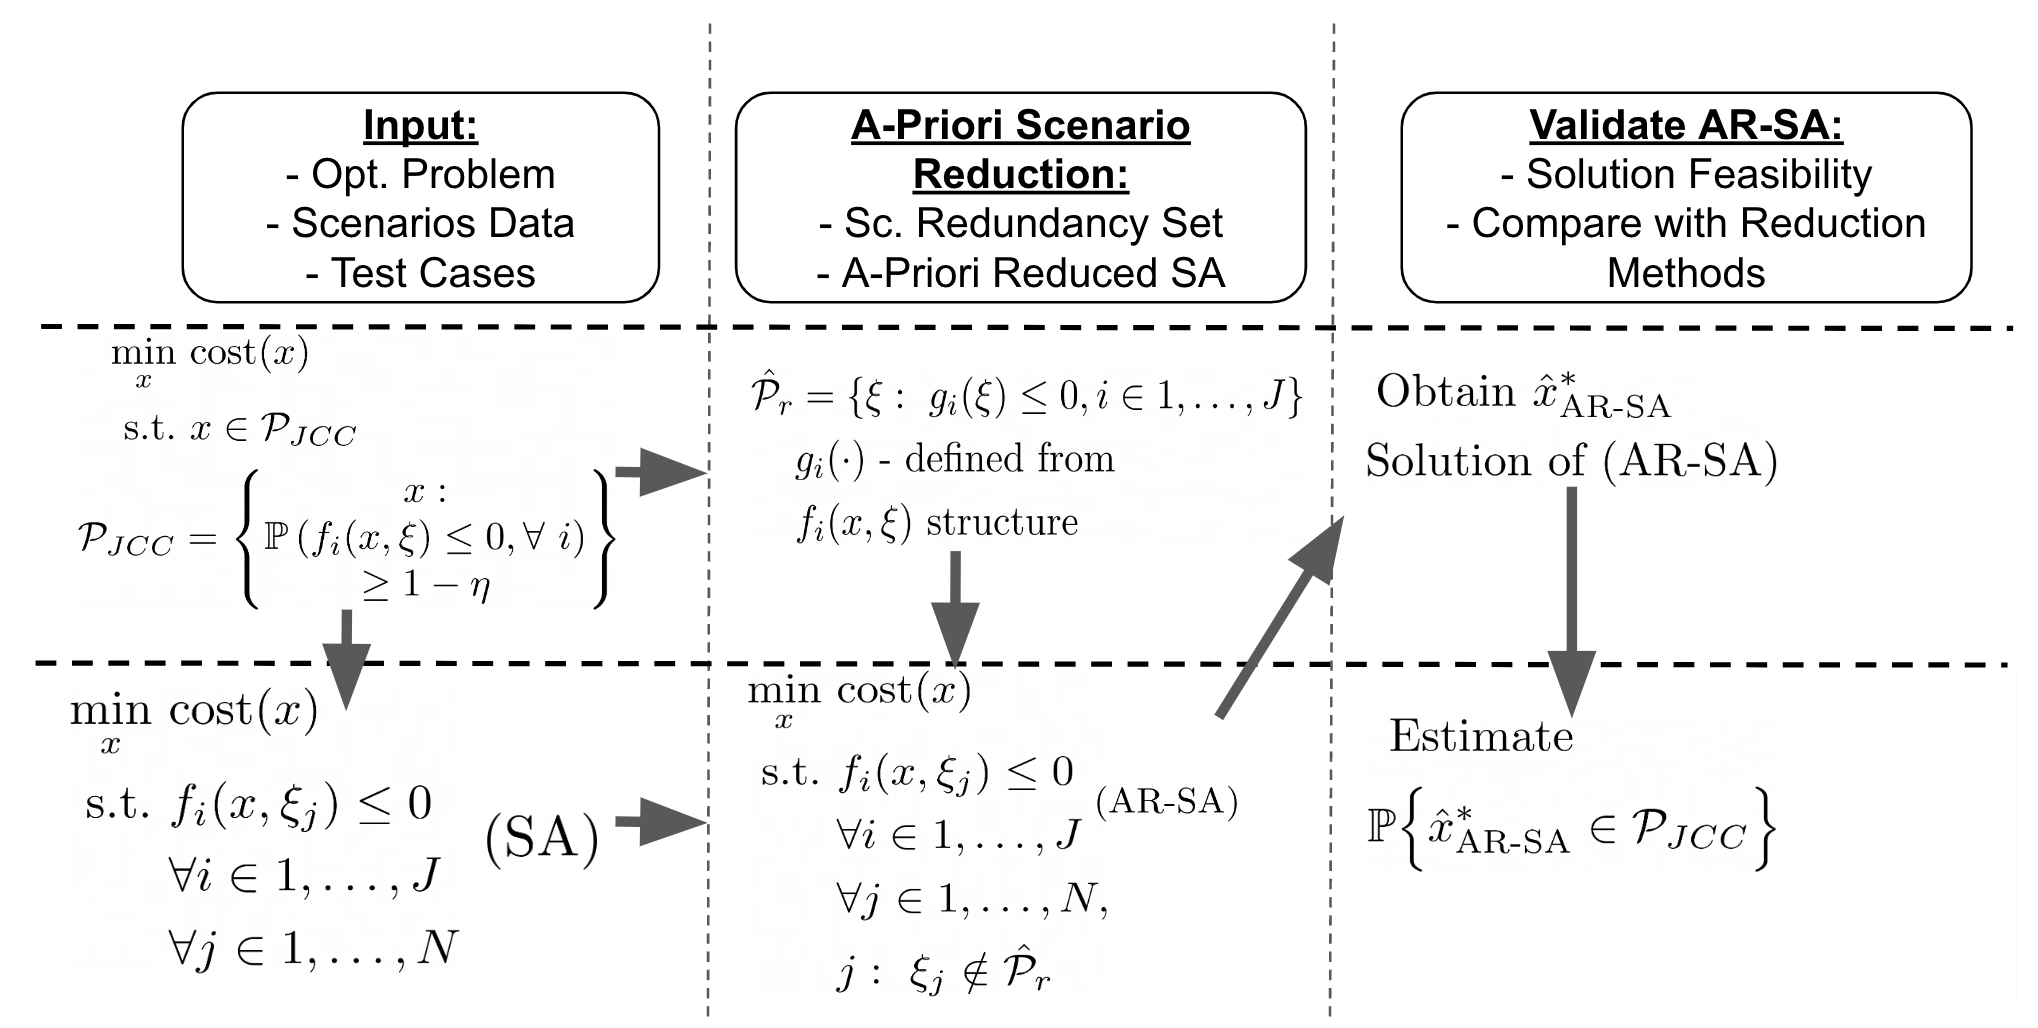
\includegraphics[width=1.\textwidth]{Dissertation/images/dynamic//scheme.png}
    \caption{AR-SA workflow.}
    \label{fig:workflow}
    \vspace{-1mm}
\end{figure}


Section 5.2 recalls the DC-OPF problem and discusses the source of uncertainty and Automated Generation Control (AGC) algorithm to balance the generation-demand mismatch. The AGC recourse adjusts the generation to a new setpoint $p^{t+1} = p^t + \alpha \xi^t$ \cite{roald2017chance,baros2021examining,mezghani2020stochastic} with $p^t \in \mathbb{R}^{n_g}$, $\alpha \in \mathbb{R}^{n_g}$, and $\xi^t \in \mathbb{R}$ representing the \emph{total} demand-generation imbalance.
The total system imbalance $\xi^{t}$ results from the combined power fluctuations due to renewable generation intermittency, demand instability, and intra-day electricity trading. Specifically, for a power system with nodes $\mathcal{B}$, the imbalance is given by $\xi^t = \sum_{b \in \mathcal{B}} (\xi_b^d)^t - (\xi_b^g)^t$, where $(\xi_b^d)^t$ and $(\xi_b^g)^t$ are random variables representing fluctuations in demand and generation at bus $b$ at time $t$, respectively. These random variables follow different distributions depending on their sources. For example, if bus $b$ has a PV generator, $(\xi_b^g)^t$ follows a beta distribution \cite{wang2010probabilistic}. For wind farms, the wind speed follows a Weibull distribution, although power output can vary among turbines \cite{dhople2012framework}. However, $\xi^t$, as the sum of random variables, follows a Gaussian distribution due to the Lyapunov or Lindeberg-Feller Central Limit Theorem \cite{scholz2011central}, \cite{rouaud2013probability, draper2021practical}.

We validated this Gaussian assumption by applying the Shapiro-Wilk normality test \cite{shapiro1965analysis} to the time series of load-renewable generation imbalance estimated from RTS-GLMC data \cite{barrows2019ieee}. This project includes time series data for demand, hydro, rooftop PV, PV, and wind farm generations. The Shapiro-Wilk test indicated that, at a significance level of $\alpha=0.05$, the null hypothesis $H_0$ (the generation-demand imbalance is normally distributed) was rejected only for August and November. Therefore, the assumption that $\xi^t$ is Gaussian is valid.
We further consider the stacked temporal uncertainty vector $\xi = (\xi^1, \dots, \xi^T) \sim \mathcal{N}(\mu, \Sigma)$, with $\Sigma$ modeling temporal correlations.

Section 5.3 ensures that AGC keeps the system balances by checking sequential timestamps and power balance.

Section 5.4 formalizes the JCC formulation for multistep DC-OPF with AGC:
\begin{align}
        & \hspace{32mm} \min_{p^t, \alpha} \mathbb{E} \sum_{t=1}^T c(p^t) \label{eq:optimal_control}, \qquad \texttt{s.t.:} 
        \\ 
        & \; \mathbb{P} 
        \begin{pmatrix}
                Wp^t \leq b, p^t = p^{t-1} + \alpha\xi^t, |p_k^t - p_k^{t-1}| \leq R_k,\\
                 1 \leq k \leq n_g, ~1\leq t \leq T
        \end{pmatrix} \geq 1 - \eta.\nonumber
\end{align}
where $\eta\in (0, 1/2]$, $\mathbb{P}$ is a joint measure induced by the uncertainty distribution, and $\alpha \in \mathbb{R}^{n_g}$ is participation factors.

A compact statement of the Problem \eqref{eq:optimal_control} is:
%assuming no uncertainty for $t = 0$:
\vspace{-3mm}
\[\min_{p^t, \alpha} \mathbb{E} \sum_{t=1}^T c(p^t) \]
\vspace{-3mm}
\begin{equation}
    \begin{aligned}
        \!\!\texttt{s.t.:}  & \mathbb{P}\!\! 
        \begin{pmatrix}
                \mathcal{W}^p p^0 + E^\tau \mathcal{W}^{\alpha} \cdot \alpha \leq \beta, 0 \leq \tau \leq T 
        \end{pmatrix}\!\geq\!1 - \eta,\!\!\!
    \end{aligned}
    \label{eq:optimal_control_2} 
\end{equation}

Next, after simplifications for further analysis, grouping all of the constraints, the SA is presented:

 \begin{align}
        & \qquad \min_{p^0, \alpha} c(p^0), \qquad \texttt{s.t.:}  \label{eq:optimal_control_sampling_02} 
        \\ 
         \forall j, 1\leq j \leq N\!\!:& \;  \mathcal{W}^p p^0 +  (E^\tau)^\top \xi(j) \mathcal{W}^{\alpha} \alpha \leq \beta, 0 \leq \tau \leq T.\nonumber
        %\end{pmatrix} \geq 1 - \eta.
\end{align}

which is built on scenarios, or data samples, $\xi(j)$, $1\le j \le N$ incapsulated in matrices $E^\tau(j)$.

Section 5.5 Discusses a-priori scenario redundancy which is illustrated in Figure \ref{fig:idea}:

\begin{definition}
\label{def:redundant}
% Consider SA \eqref{eq:optimal_control_sampling_02} that has a solution $(\hat{p}^0_{\mathcal{I}}, \hat{\alpha}_{\mathcal{I}})$ which is feasible for the JCC problem \eqref{eq:optimal_control_2} and a set of scenarios~$\mathcal{I}$. An set of scenarios ${\cal I}_r$ is redundant iff it does not change the solution, $(\hat{p}^0_{\mathcal{I}}, \hat{\alpha}_{\mathcal{I}}) = (\hat{p}^0_{\mathcal{I} \setminus \mathcal{I}_r}, \hat{\alpha}_{\mathcal{I} \setminus \mathcal{I}_r})$.
Let $\mathcal{I} = \{1, \dots, N\}$. Scenarios indexed with $\mathcal{I}_r \subset \mathcal{I}$ are called redundant iff a solution of SA with constraints corresponding to scenarios indexed with $\mathcal{I}_r$ are omitted - $(\hat{p}^0_{\mathcal{I} \setminus \mathcal{I}_r}, \hat{\alpha}_{\mathcal{I} \setminus \mathcal{I}_r})$ - is feasible for initial JCC \eqref{eq:optimal_control_2} and solution of SA $(\hat{p}^0_{\mathcal{I}_r}, \hat{\alpha}_{\mathcal{I}_r})$ with constraints corresponding to those scenarios indexed with $\mathcal{I}_r$ is not feasible for JCC \eqref{eq:optimal_control_2}.
\end{definition}

\def\shift{2.7}
\def\shiftt{2.}
\def\shiftuselesssample{0.3}
\def\shiftusefulsample{1.1}
\def\xx2{0 + \shiftt}
\def\yx2{0 - \shiftt}
\def\threshold{33} 
\tikzset{snake it/.style={decorate, decoration={coil,amplitude=1pt, segment length=9pt}}}
\begin{figure}
\begin{minipage}{0.35\linewidth}
    \centering
        \begin{tikzpicture}[scale=0.55, node distance={15mm}, thick, main/.style = {draw, scale=.5}] 
        \clip (0,2) rectangle + (6,-7);
        
        \coordinate (x2) at (\xx2, \yx2);
        \coordinate (x2origin) at (\xx2 + 1.5, \yx2 - 2);
        \draw[olive] (x2) circle (1pt);
        \draw (x2) ++(1.5, -2.3) node[olive, above right] (tmp) {$(\hat{p}_{\mathcal{I}}, \hat{\alpha}_{\mathcal{I}})$};
        \draw[->, olive] (x2origin) -- (x2);
        %Deterministic set - outer guy
        \coordinate (a) at ( 4.755282581475767 , 1.545084971874737 );
        \coordinate (b) at ( 3.061616997868383e-16 , 5.0 );
        \coordinate (c) at ( -4.755282581475767 , 1.5450849718747375 );
        \coordinate (d) at ( -2.9389262614623664 , -4.045084971874736 );
        \coordinate (e) at ( 2.9389262614623646 , -4.045084971874738 );
        %linking outer guy
        \draw (a) -- (b);
        \draw (b) -- (c);
        \draw (c) -- (d);
        \draw (d) -- (e);
        \draw (e) -- (a);
        %annotating outer guy
        \draw
        (a) ++(0.1, -1.21) node[below] (tmp) {$P$};
        %(tmp.west) -- (PO);
        
        %JCC feasibility set - green guy
        \coordinate (ag) at ( 3.804226065180614 , 1.2360679774997896 );
        \coordinate (bg) at ( 2.4492935982947064e-16 , 4.0 );
        \coordinate (cg) at ( -3.804226065180614 , 1.23606797749979 );
        \coordinate (dg) at ( -2.351141009169893 , -3.2360679774997894 );
        \coordinate (eg) at ( 2.3511410091698917 , -3.2360679774997902 );
        %linking green guy
        \draw [black, snake it] (ag) -- (bg);
        \draw [black, snake it] (bg) -- (cg);
        \draw [black, snake it] (cg) -- (dg);
        \draw [black, snake it] (dg) -- (eg);
        \draw [black, snake it] (eg) -- (ag);
        %annotating green guy
        \draw
        (ag) ++(0., -0.6) node[left, black] (tmp) {${P}_{\textup{JCC}}$};
        %(tmp.west) -- (PO);
        
        %Redundant samples botder - teal
        \coordinate (ar2) at ( 0.9510565162951535 + \shiftt , 0.3090169943749474 - \shiftt);
        \coordinate (br2) at ( 6.123233995736766e-17 + \shiftt , 1.0  - \shiftt);
        \coordinate (cr2) at ( -0.9510565162951535  + \shiftt, 0.3090169943749475  - \shiftt);
        \coordinate (dr2) at ( -0.5877852522924732 + \shiftt, -0.8090169943749473 - \shiftt);
        \coordinate (er2) at ( 0.5877852522924729 + \shiftt, -0.8090169943749476  - \shiftt);
        %linking teal
        \draw [teal, snake it] (ar2) -- (br2);
        \draw [teal, snake it] (br2) -- (cr2);
        \draw [teal, snake it] (cr2) -- (dr2);
        \draw [teal, snake it] (dr2) -- (er2);
        \draw [teal, snake it] (er2) -- (ar2);
        %annotating teal guy
        \draw
        (br2) ++(1em, .1em) node[above, teal] (tmp) {$\mathcal{P}_{r}$};
        %(tmp.west) -- (PO);

        %Inner redundant - purple
        \coordinate (anvc) at ( 0.9510565162951535 * 0.7 + \shiftt , 0.3090169943749474 * 0.7 - \shiftt);
        \coordinate (bnvc) at ( 6.123233995736766e-17 + \shiftt , 1.0 * 0.7  - \shiftt);
        \coordinate (cnvc) at ( -0.9510565162951535 * 0.7  + \shiftt, 0.3090169943749475 * 0.7  - \shiftt);
        \coordinate (dnvc) at ( -0.5877852522924732 * 0.7 + \shiftt, -0.8090169943749473 * 0.7 - \shiftt);
        \coordinate (envc) at ( 0.5877852522924729 * 0.7 + \shiftt, -0.8090169943749476 * 0.7  - \shiftt);
        %linking purple
        \draw [purple] (anvc) -- (bnvc);
        \draw [purple] (bnvc) -- (cnvc);
        \draw [purple] (cnvc) -- (dnvc);
        \draw [purple] (dnvc) -- (envc);
        \draw [purple] (envc) -- (anvc);
        %annotating purple
        \draw
        (envc) ++(3.3em, .3em) node[above, purple] (tmp) {$\hat{\mathcal{P}}_{r}$};

        % %NNR - necessarily redundant
        % \coordinate (annr) at ( 0.9510565162951535 * 1.3 + \shiftt , 0.3090169943749474 * 1.3 - \shiftt);
        % \coordinate (bnnr) at ( 6.123233995736766e-17 + \shiftt , 1.0 * 1.3  - \shiftt);
        % \coordinate (cnnr) at ( -0.9510565162951535 * 1.3  + \shiftt, 0.3090169943749475 * 1.3  - \shiftt);
        % \coordinate (dnnr) at ( -0.5877852522924732 * 1.3 + \shiftt, -0.8090169943749473 * 1.3 - \shiftt);
        % \coordinate (ennr) at ( 0.5877852522924729 * 1.3 + \shiftt, -0.8090169943749476 * 1.3  - \shiftt);
        % %linking red guy
        % \draw [brown] (annr) -- (bnnr);
        % \draw [brown] (bnnr) -- (cnnr);
        % \draw [brown] (cnnr) -- (dnnr);
        % \draw [brown] (dnnr) -- (ennr);
        % \draw [brown] (ennr) -- (annr);
        % %annotating red guy
        % \draw
        % (cnnr) ++(-1.3em, .3em) node[above, brown] (tmp) {$\overline{P_{r}}$};
        
        %% Generate in loop and colorize based on distance to x*
        \pgfmathsetmacro{\xRange}{1.3} % adjust range as needed
        \pgfmathsetmacro{\yRange}{1.3} % adjust range as needed
        \pgfmathsetseed{3}
        \foreach \i in {1,...,30} {
            
            \def\xrandom{\shiftt + rand*\xRange}
            \def\yrandom{-\shiftt + rand*\yRange}
        
            \filldraw [black] (\xrandom, \yrandom) circle (1pt);
            
        }
        \end{tikzpicture}  
        \end{minipage}
            \hfill % Adds horizontal space between the minipages
        \begin{minipage}{0.65\linewidth}
        \vspace{-3mm}
            \begin{itemize}
                \item $P$ is a feasibility set
                \item $P_{\textup{JCC}}$ is a JCC feasibility set
                \item The black dots -- potential setpoints achievable by the AGC due to power fluctuations
                \item $(\hat{p}_{\mathcal{I}}, \hat{\alpha}_{\mathcal{I}})$ is the SA solution based on all data samples
            \end{itemize}
        \end{minipage}
        % \vspace{-6mm}
    \caption{%Let  $P$ and $P_{\textup{JCC}}$ be (non-convex) deterministic feasibility and JCC feasibility sets resp. 
    %The black dots represent potential setpoints achievable by the AGC due to fluctuations. 
    %Based on all data samples, one can solve SA and get a solution $(\hat{p}_{\mathcal{I}}, \hat{\alpha}_{\mathcal{I}})$. 
    All data samples can be divided into redundant and non-redundant, depending on whether they are inside or outside the set $\mathcal{P}_r$ with an unknown structure. In practice, one can derive inner approximations $\hat{\mathcal{P}}_r$ of $\mathcal{P}_r$. The latter can be used to classify data by redundancy in SA.}
    \label{fig:idea}
  %\vspace{-4mm}
\end{figure}

The standard assumption is applied: 
\begin{assumption}\label{asmp:dyn_10}
For all possible uncertainty realizations $\xi(1), \dots, \xi(N)$, optimization problem \eqref{eq:optimal_control_sampling_02} is either infeasible or has a unique optimal solution.
\end{assumption}

% Next, technical lemma and corollary are presented:
% \begin{lemma}
%     \label{lemma:bound_prob}
%      Let $\pi(p^0, \alpha) \geq 1 -\eta$, where $$\pi(p^0, \alpha) = \mathbb{P}\left\{ \cap_{i, \tau} (\omega^p_i)^\top p^0 + (E^\tau_i)^\top \xi \cdot(\omega^\alpha_i)^\top \alpha \leq \beta_i\right\}.$$ Then 
%     \vspace{-2mm}
%     \[\max_{i, t} \mathbb{P} \left\{ (\omega^p_i)^\top p^0 + (E^\tau_i)^\top \xi \cdot (\omega^\alpha_i)^\top \alpha > \beta_i \right\} \leq 1-\pi(p^0, \alpha).\]
% \end{lemma}

The redundancy theorem is stated and proven
\begin{theorem}
Let scenarios $\xi(j) \sim \mathcal{N}(0, \Sigma), ~ j \in \mathcal{I}=\{1, \dots, N\}$ form SA \eqref{eq:optimal_control_sampling_02} and a solution of this problem $(\hat{p}^0_{\mathcal{I}}, \hat{\alpha}_{\mathcal{I}})$ be feasible for the JCC problem \eqref{eq:optimal_control_2}. Moreover, assume that the cost function $c(\cdot)$ is linear.  Let $\hat{\mathcal{P}}_r = \{ \xi\in \mathbb{R}^T:~ |(E^{\tau}_i)^\top \xi|  \leq \Phi^{-1}(1 - \eta) \sigma^\tau_i \gamma ~\forall i, \tau \}$, where $\gamma \in (0, 1)$ and $(\sigma^\tau_i)^2 = (E^\tau_i)^\top \Sigma (E^\tau_i)$.
Then, first, SA  where scenarios $\xi(j), ~ j \in \mathcal{I}_r = \{ j: \xi(j) \in \hat{\mathcal{P}}_r \}$ yields solution $(\hat{p}^0_{\mathcal{I}_r}, \hat{\alpha}_{\mathcal{I}_r})$ that is not feasible for original JCC Problem \eqref{eq:optimal_control_2}. Second, SA where scenarios $\xi(j), ~ j \in \mathcal{I} \setminus \mathcal{I}_r$ yields the solution $(\hat{p}^0_{\mathcal{I} \setminus \mathcal{I}_r}, \hat{\alpha}_{\mathcal{I} \setminus \mathcal{I}_r})$ that is feasible for the original JCC Problem \eqref{eq:optimal_control_2}.
\label{th:P_r sampling polytope}
\end{theorem}

Theorem \ref{th:P_r sampling polytope} establishes a sufficient, a priori condition on sample redundancy within a dataset $\xi(j), j \in \mathcal{I}$ that guarantees a feasible solution. Specifically, if a dataset can ensure a feasible solution for the original JCC problem, samples within $\hat{\mathcal{P}}_r$ can be disregarded. This theorem provides a way to evaluate the dataset's potential beforehand: if all data samples fall within $\mathcal{P}_r$, it is impossible to derive a feasible solution for the JCC from this data.
% \begin{corollary}
%     \label{lemma:corollary}
%     Let $(p^0, \alpha)$ be feasible to JCC in \eqref{eq:optimal_control_2}. Then $$\max_{i, t} \mathbb{P} \left\{ (\omega^p_i)^\top p^0 + (E^\tau_i)^\top \xi \cdot (\omega^\alpha_i)^\top \alpha > \beta_i \right\} \leq \eta.$$
% \end{corollary}
The next theorem finishes the section with guarantees on the data complexity (number of scenarios required to get $1-\rho$ reliable approximate solution) of the AR-SA:

\begin{theorem}\label{thm:dyn_40}
Let $(\hat{p}^0, \hat{\alpha})$ be a unique solution of the SA Problem~\eqref{eq:optimal_control_sampling_02} with $N$ i.i.d. samples, so that none of the samples belong to $\hat{\mathcal{P}}_{r}$. Moreover, assume that for any $N$ the assumption \ref{asmp:dyn_10} is fulfilled. Then for any $\rho \in (0,1)$ and any~$\eta \in (0, 1/2]$, $(\hat{p}^0, \hat{\alpha})$ is also a solution for the Chance-constrained optimal power flow Problem~\eqref{eq:optimal_control_2} with probability at least $1-\rho$ if 
$%\begin{align*}
  N \ge \left\lceil 2\eta^{-1}(1-\nu)\ln \frac{1}{\rho} + 2d + 2d\eta^{-1}(1-\nu) \ln\frac{2(1-\nu)}{\eta} \right\rceil, 
$%\end{align*} 
 where $d$ is a dimension of the space of controllable generators and participation factors, i.e., $d = 2 n_g$, and $\nu$ is the probability of a random scenario $\xi \sim \mathcal{N}(0, \Sigma)$ to belong to $\hat{\mathcal{P}}_{r}$, and $\nu < 1$. 
\end{theorem}

Section 5.6 provides numerical experiments on power grids. It compares Data-Driven Distributionally Robust Optimization approach, other a-priori scenario reduction methods such as Simultaneous Backward, Fast Forward and K-Means Clustering methods with AR-SA. 
%For estimating the reliability, it uses the same algorithm as in previous Chapter, i.e., Algorithm \ref{alg:estimate_delta} for $\rho$.
We also compared the execution time of the algorithms empirically and compared asymptotic complexities.

Regarding the complexities, the Fast Forward method adds scenarios incrementally based on probabilistic metrics (2-Wasserstein distance) and adjusts probabilities after each addition. Conversely, the Simultaneous Backward method removes scenarios using the same process. For a target number of scenarios $N_r$, the complexities of these methods are $O(N_r^3 + N_r N^2)$ and $O(N_r^3 + N^3)$, respectively \cite{heitsch2003scenario, rujeerapaiboon2022scenario}.

The K-Means algorithm, which involves iterative estimation of scenario cluster centers and $L_2$ distance calculation between scenarios and cluster centers, has a complexity of $O(N_rN^2)$ \cite{pakhira2014linear}. In contrast, the proposed AR-SA method reduces scenarios by checking if the current samples are within $\hat{\mathcal{P}}_r$, resulting in a complexity of $O(N)$. The construction of $\hat{\mathcal{P}}_r$ itself grows linearly with the number of deterministic constraints under the probability measure in the JCC.
The empirical comparison is given in Figures below and in Table \ref{tab:dyn_summary_results}

\begin{table}[t]
\caption{The number of samples for AR-SA and SA required in CC-OPF with a confidence threshold of $1-\eta$ to get the empirical reliability of $1-\hat{\rho} = 0.99$. The value of $1-\eta$ is given by out-of-sample Monte Carlo; the empirical reliability is given by averaging over $L=100$ independent CC-OPF problem instances. 
    }
    \centering
        % \begin{tabular}{lrr|lr|ll}
        \begin{tabular}{|lr|rlrll|}
        \toprule
        Case & $\eta$ & SA & AR-SA & SA-FF & SA-SB & SA-KMeans \\
\midrule
grid14 & 0.05 & 93 & 48 & 48 & 138 & 48 \\
grid30 & 0.05 & 138 & 93 & 138 & 138 & 93 \\
grid14 & 0.01 & 363 & 93 & 363 & 363 & 363 \\
grid30 & 0.01 & 453 & 273 & 453 & 453 & 453 \\
\bottomrule
        \end{tabular}
    
    
    \label{tab:dyn_summary_results}
\end{table}

% \begin{figure}[hbt]
% % \vspace{-15mm}
% % \begin{minipage}[b]{.99\textwidth}
% \begin{subfigure}{.50\textwidth}
%   \centering
%   % include second image
%   \hspace{-0mm}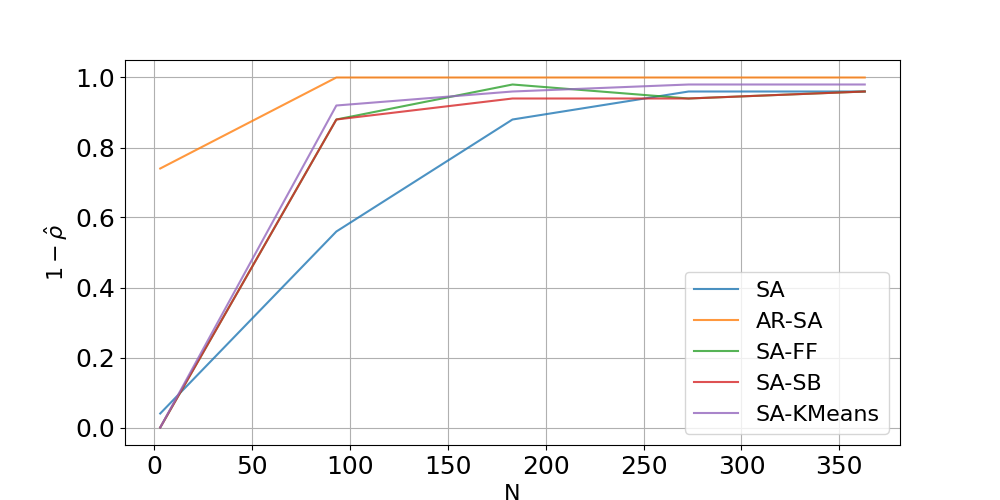
\includegraphics[width=0.95\linewidth]{Dissertation/images/dynamic/washington14/1_beta_N_363_eta_0.01.png}
%   \caption{Empirical reliability %$(1-\hat{\rho})$ 
%   vs. $\#$ samples in CC-OPF for Washington 14 bus, $\eta = 0.01$.}
%   \label{fig:washington14conservatism}
% \end{subfigure}
% \begin{subfigure}{.50\textwidth}
%   \centering
%   % include second image
%   \hspace{-0mm}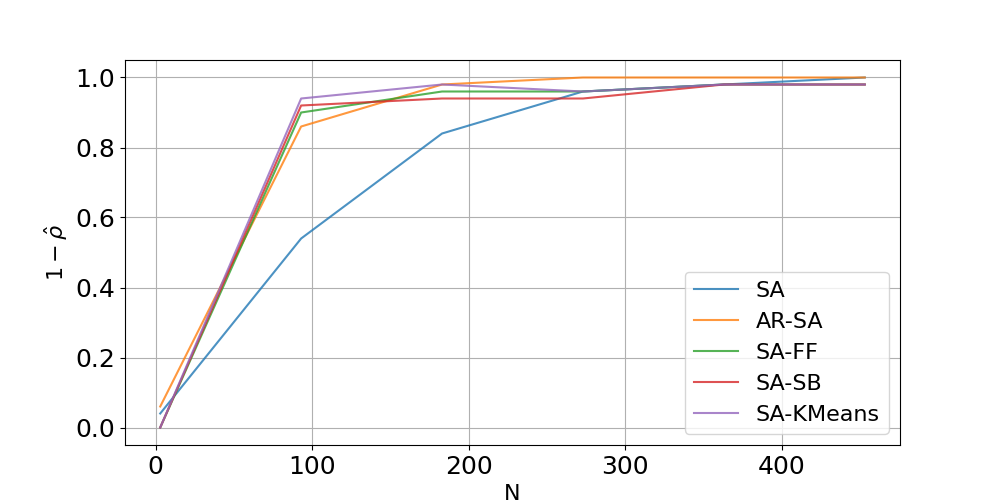
\includegraphics[width=0.95\linewidth]{Dissertation/images/dynamic/ieee30/1_beta_N_453_eta_0.01.png}
%   \caption{Empirical reliability %($1-\hat{\rho}$) 
%   vs $\#$ samples  in CC-OPF for IEEE 30 bus system, $\eta = 0.01$.}
%   \label{fig:ieee30conservatism}
% \end{subfigure}\\
% \begin{subfigure}{.50\textwidth}
%   \centering
%   % include second image
%   \hspace{0mm}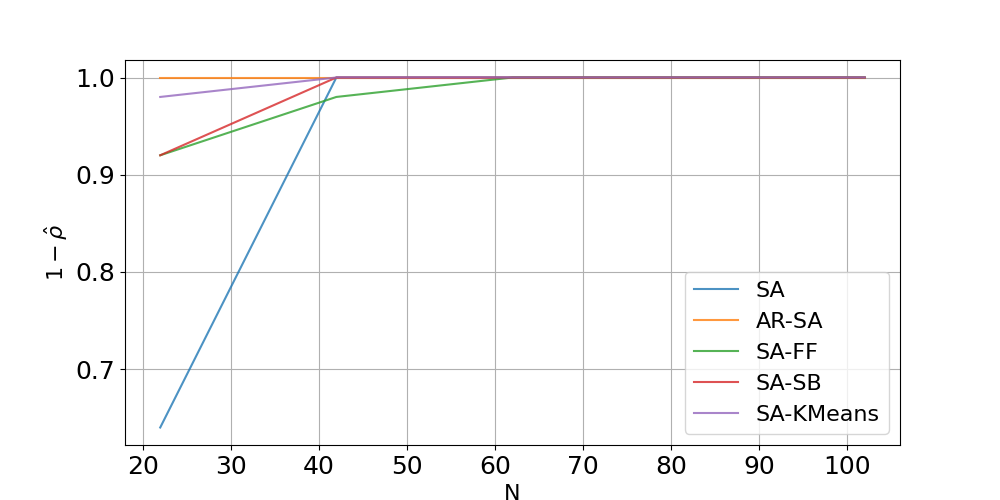
\includegraphics[width=0.95\linewidth]{Dissertation/images/dynamic/grid6/1_beta_N_102_eta_0.1.png}
%   \caption{Empirical reliability %($1-\hat{\rho}$) 
%   vs $\#$ samples  in CC-OPF for Grid6-WW 6 bus system, $\eta = 0.1$.}
%   \label{fig:grid6reliability}
% \end{subfigure}
% \begin{subfigure}{.50\textwidth}
%   \centering
%   % include second image
%   \hspace{0mm}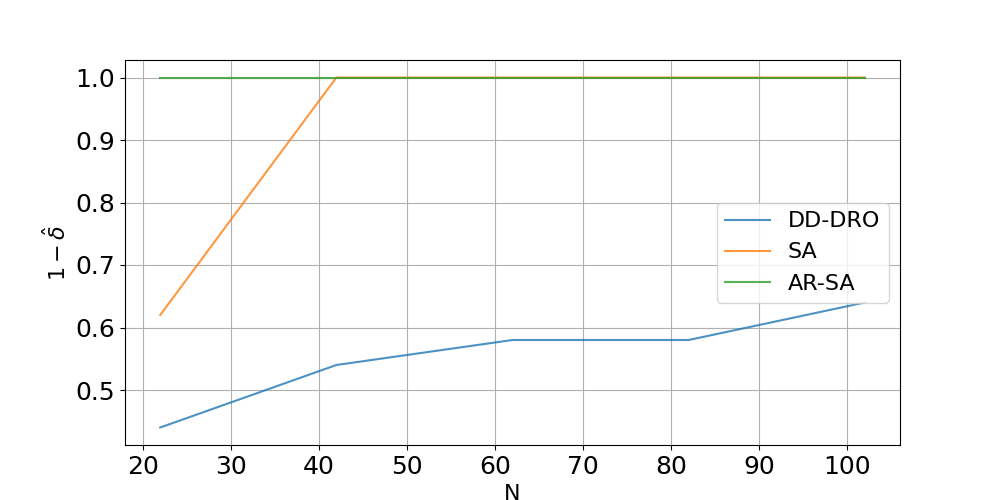
\includegraphics[width=0.95\linewidth]{Dissertation/images/dynamic/grid6/dd-dro/1_beta_N_102_eta_0.1.png}
%   \hspace{0mm}\caption{Empirical reliability  
%   vs $\#$ samples  in CC-OPF for Grid6-WW 6 bus system, $\eta = 0.1$.}
%   \label{fig:grid6reliability-dd-dro}
% \end{subfigure}

% \begin{subfigure}{.50\textwidth}
%   \centering
%   % include first image
% \hspace{10mm}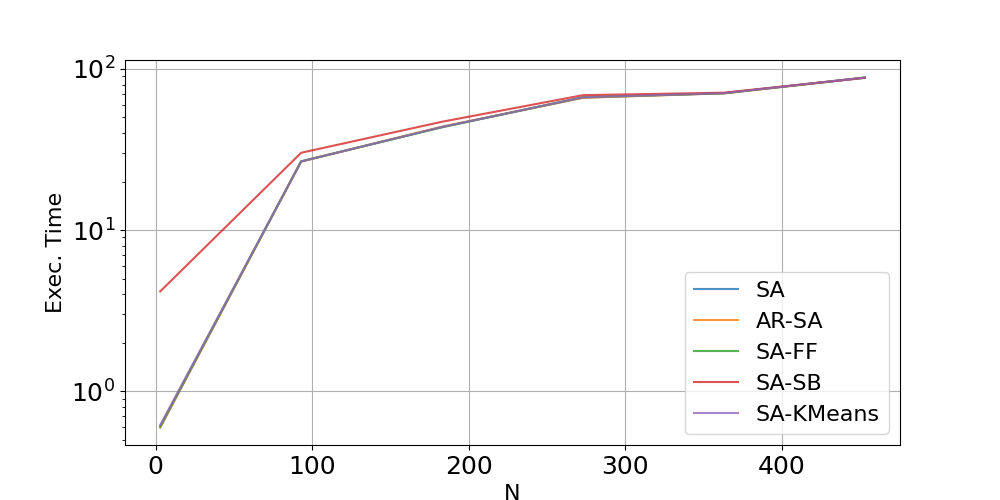
\includegraphics[width=0.95\linewidth]{Dissertation/images/dynamic/ieee30/exec_time_N_453_eta_0.01.png}~~~~~~\hfill
%   \caption{Exec. time vs $\#$ samples, IEEE 30 bus, $\eta = 0.01$.
%   }
%   \label{fig:ieee30time}
% \end{subfigure}
% \begin{subfigure}{.50\textwidth}
%   \centering
%   % include first image
% \hspace{10mm}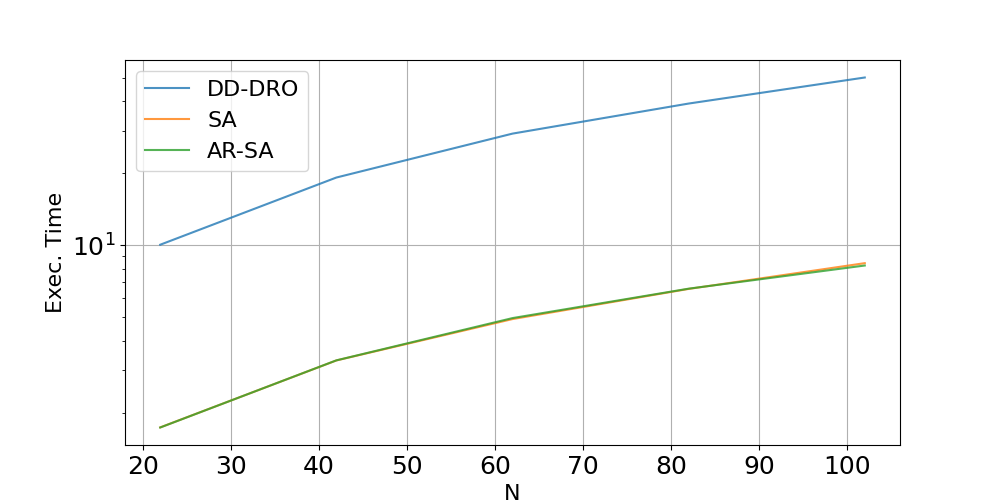
\includegraphics[width=0.95\linewidth]{Dissertation/images/dynamic/grid6/dd-dro/exec_time_N_102_eta_0.1.png}~~~~~~\hfill
%   \caption{Exec. time vs $\#$ samples, Grid6-WW bus, $\eta = 0.1$.
%   }
%   \label{fig:grid6time-dd-dro}
% \end{subfigure}

% \vspace{-7mm}

% \caption{(a, b, d) Empirical reliability ($1-\hat{\rho}$). (e, c, f) Execution time for IEEE-30 and Grid6-WW. The empirical estimates are computed with $L = 200$ optimization instances (for $1-\hat{\rho}$), and $N_{MC}=10^4$ Monte-Carlo samples for each instance to determine constraint validation (for box-plot of $(\hat{\mathbb{P}}_N)_l$).  
% }
% \label{fig:dyn_ieee118}
% \end{figure}

% \newpage

Finally, the chapter concludes in Secion 5.7. Data-driven approximations are beneficial for chance-constrained stochastic programs with unknown uncertainty distributions or JCC settings. However, data demands can quickly become unmanageable with increasing size and reliability requirements. To address this, we proposed a novel method to identify and eliminate redundant scenarios in stochastic approximations for JCC dynamic multi-timestamp DC-OPF. We validate this approach theoretically and demonstrate its high empirical performance across various test cases.

% The \textbf{conclusions chapter} summarizes the thesis consolidates the presented results and offers a concise summary of the investigation’s significance
\section*{Conclusion}
\begin{enumerate}
    \item The adaptive importance sampling algorithm combined with the mirror descent optimization method for usage in power systems has been proposed. The use case is the estimation of the current generation regime's reliability against Gaussian perturbations.
        The algorithm's convergence and validity have been proven theoretically by stating and demonstrating a convergence theorem for optimizing the estimate's variance. The theoretical result underscores algorithm efficiency with $O\left( \sqrt{\log J} \right)$ scaling for the number of constraints $J$.
        The effectiveness and potential advantages of this novel approach have been demonstrated by providing an extensive comparison of its performance with practical algorithms, such as pmvnorm and ALOE, in power systems. Further development in this direction exists as well. The algorithm can be generalized to non-linear settings by using a sampling technique in the complement of convex sets (Grid Walk, Rejection Sampling) and using convex restrictions, see, e.g., \cite{lee2019convex}.
        
    \item A new, significantly more efficient method for constructing scenario approximations has been proposed in the case of Gaussian additive uncertainty with application to power systems optimization - OPF, which is a fundamental routine for operating a power grid. The theoretical guarantees for this new method have been proven. They ensure its mathematical soundness and reliability, indicating a sound reduction in data samples, i.e., scenario usage in scenario approximations in comparison to proven classical results. The performance of the new scenario approximation method in power systems has been demonstrated by comparing it with classical Monte Carlo-based approaches to highlight its data efficiency and accuracy in providing solutions for Joint Chance-Constrained (JCC) problems which are known to have no analytical formulation in general, requiring on average 2 times less data samples (scenarios) than classical approaches. Further prospects in this direction include generalization to non-linear settings, keeping uncertainties' additivity.
    \item An a priori approach to reduce the size of scenario approximations for non-Gaussian multiplicative uncertainty in the setting of dynamic optimal power flow with automatic generation control (AGC) has been proposed. The proposed approach has greatly enhanced computational efficiency and accuracy of the resulting reduced scenario approximation. 
    %Also, the normality of generation-demand mismatch using real time series data from various sources of load and renewable generation
    The effectiveness and reliability of this a priori approach have been confirmed by proving formal statements on its validity in reducing scenario approximations.
    The superior performance and practical applicability of this a priori approach have been demonstrated by comparing it with other scenario reduction methods, including data-driven distributional robust optimization. The experiments have shown that the proposed approach allows to reduce up to a half of scenarios without corrupting the scenario approximation and does not introduce additional exhaustive computations. The further developments can be applications and generalization to a non-linear setting for multiplicative uncertainty.
\end{enumerate}